\documentclass[11pt,a4paper]{report}

% ============== Page Setup ==============
\usepackage[a4paper,top=2.5cm,bottom=2.5cm,left=2.5cm,right=2.5cm]{geometry}

% ============== Packages ==============
\usepackage{graphicx}
\usepackage{float}
\usepackage{tikz}
\usetikzlibrary{calc}
\usepackage{setspace}
\usepackage[nottoc]{tocbibind}
\usepackage{acronym}
\usepackage{booktabs}
\usepackage{multirow}
\usepackage{amsmath}
\usepackage{amssymb}
\usepackage{caption}
\usepackage{subcaption}
\usepackage[hidelinks]{hyperref}
\usepackage[backend=biber,style=ieee]{biblatex}
\addbibresource{references.bib}

% ============== Typography / Spacing ==============
\setstretch{1.15}
\setlength{\parskip}{6pt}
\setlength{\parindent}{0pt}

% ============== Custom Commands ==============
\newcommand{\figwidth}{0.85\textwidth}

\begin{document}

% ======================= COVER PAGE ==========================
\begin{titlepage}
\thispagestyle{empty}
\centering
\begin{tikzpicture}[remember picture, overlay]
  \draw[line width=0.8pt]
    ($(current page.north west) + (2cm,-2cm)$)
    rectangle
    ($(current page.south east) + (-2cm,2cm)$);
\end{tikzpicture}

{\bfseries\large UNIVERSITY OF SCIENCE AND TECHNOLOGY OF HANOI\par}
\vspace{4pt}
{\bfseries\large DEPARTMENT OF INFORMATION AND COMMUNICATION TECHNOLOGY\par}

\vspace{2.4cm}
\IfFileExists{figures/logo.png}{
  
\includegraphics[width=6cm]{figures/logo.png}\par
}{
  \vspace*{3.5cm}
}
\vspace{1.8cm}

{\bfseries\Large BACHELOR'S THESIS REPORT\par}
\vspace{10pt}
{\bfseries\Large Automatic Recognition of Surgical Phases in Cholecystectomy Videos: A Comparison of Three Modern Deep-Learning Architectures on Cholec80\par}

\vspace{2.0cm}
\begin{tabular}{@{}rl@{}}
\textbf{Submitted by:} & Nguyen Trong Bach\\[10pt]
\textbf{Supervisor:} & Dr. Vu Trong Sinh\\
\end{tabular}

\vfill
{\large June 2026\par}
\end{titlepage}

% ======================= ACKNOWLEDGEMENTS ==========================
\chapter*{Acknowledgements}
\addcontentsline{toc}{chapter}{Acknowledgements}

First and foremost, I would like to express my sincere gratitude to my supervisor, Dr.~Vu Trong Sinh, for his invaluable guidance, continuous support, and deep knowledge of medical imaging. His practical insights and constructive feedback shaped the direction of this work and substantially improved its quality.

I am grateful to the CAMMA research group at the University of Strasbourg for releasing the Cholec80 dataset, without which this study would not have been possible, and to the open-source community behind PyTorch, timm, and scikit-learn, whose tools underpin every experiment reported here.

Finally, I want to thank my family for their unconditional love and unwavering belief in me throughout the long nights of training and debugging. I dedicate this milestone to them.

% ======================= ABSTRACT ==========================
\chapter*{Abstract}
\addcontentsline{toc}{chapter}{Abstract}

Surgical phase recognition means labelling each frame of an operation video with the step that is taking place. It is a useful building block for operating-room analytics, skill assessment, and decision support. The Cholec80 dataset of eighty gallbladder-removal videos divides each operation into seven phases. The phases are very unevenly distributed---the most common one covers 42.7\% of frames while the rarest covers only 3.8\%, a ratio of about 11 to 1---and many frames near phase changes look alike, which makes the task hard.

This thesis has two parts. The first is a \textbf{fair comparison of three architectures}: ResNet-50 with a bidirectional LSTM, EfficientNet-B3 with a temporal convolutional network, and Swin-Tiny with a Transformer. All three are trained with exactly the same pipeline---a three-stage schedule, automatic class re-weighting, an extra tool-detection task, label smoothing, and mixed-precision training---so that any difference in results comes from the architecture and not from the training setup. On the held-out test set of twenty videos, the Swin-Transformer reaches a smoothed macro-F1 of \textbf{0.815} (accuracy 0.862), 3.4 points above the ResNet-LSTM and 6.7 points above the EfficientNet-TCN; combining the three models adds a small further gain. Four ablations show that the extra tool task is worth about $+1.6\%$ macro-F1 and class re-weighting about $+2.0\%$---together as large as the gap between the best and worst architecture.

The second part looks at the \textbf{decoding and calibration steps} that most Cholec80 work skips. We add a real-time decoder that uses only past frames: it combines temperature-calibrated predictions with a transition table learned from the training videos. Without retraining the models, it raises test accuracy by $+0.6$ to $+1.7$ points (paired Wilcoxon $p < 0.001$, Cohen's $d > 0.97$) at a cost of 0.013~ms per frame, with the biggest gains near phase changes. Comparing against an offline decoder that may look at the whole video shows that the remaining gap is almost entirely inside long stable phases, not at the phase changes themselves.

Overall, the thesis shows that good surgical phase recognition is possible on an ordinary laptop GPU when training, decoding, and post-processing are designed together, and that on an imbalanced dataset the training recipe matters as much as the choice of architecture.

% ======================= TOC / LOF / LOT ==========================
\tableofcontents
\listoffigures
\listoftables

% ======================= LIST OF ABBREVIATIONS ==========================
\chapter*{List of Abbreviations}
\addcontentsline{toc}{chapter}{List of Abbreviations}

\begin{acronym}[MICCAI]
\acro{AdamW}{Adam with decoupled Weight decay}
\acro{AUC}{Area Under the ROC Curve}
\acro{BiLSTM}{Bidirectional Long Short-Term Memory}
\acro{CNN}{Convolutional Neural Network}
\acro{ECE}{Expected Calibration Error}
\acro{fps}{Frames Per Second}
\acro{HMM}{Hidden Markov Model}
\acro{LSTM}{Long Short-Term Memory}
\acro{MICCAI}{Medical Image Computing and Computer Assisted Intervention}
\acro{NLL}{Negative Log-Likelihood}
\acro{TCN}{Temporal Convolutional Network}
\acro{ViT}{Vision Transformer}
\end{acronym}

% ======================= CHAPTER 1 ==========================
\chapter{Introduction}

\section{Background and Motivation}

Keyhole surgery produces a large amount of video that is recorded but rarely looked at again. A laparoscopic cholecystectomy---removal of the gallbladder---usually lasts between thirty and ninety minutes and follows a fixed sequence of steps. A system that recognises these steps automatically would help in several ways: writing operative reports, assessing the skill of trainees, estimating how much longer an operation will take, and warning the team when the workflow departs from the expected order~\cite{maierhein2017surgical,vedula2017objective}.

The Cholec80 dataset, released by the CAMMA group at the University of Strasbourg in 2017, is the standard benchmark for this task~\cite{twinanda2017endonet}. It contains eighty cholecystectomy videos recorded at 25 frames per second. Every frame is labelled with one of seven surgical phases and with which of seven instruments are visible. The seven phases---Preparation, Calot's triangle dissection, Clipping and cutting, Gallbladder dissection, Gallbladder packaging, Cleaning and coagulation, and Gallbladder retraction---always occur in the same order, a property this thesis later uses at the decoding stage.

Deep learning is the standard approach. Early systems used a single convolutional network to label each frame on its own; later work added a temporal model---recurrent, convolutional, or attention-based---trained together with the image encoder. The main difficulty, though, is not the model but the data: Cholec80 is dominated by a few long phases, so a model trained without any correction learns to predict those phases for almost everything. This gives a high frame-level accuracy while almost ignoring the short closing phases that are clinically important.

\section{Problem Statement}

Surgical phase recognition on Cholec80 is shaped by three difficulties that this thesis addresses directly.

\textbf{Class imbalance.} Calot's triangle dissection alone makes up 42.7\% of frames, while Gallbladder retraction covers only 3.8\%---a ratio above eleven to one. A model trained without correction learns to predict the common phases, and frame-level accuracy hides this because the common phases are also the easy ones.

\textbf{Comparisons that mix too many factors.} Three families of methods---CNN~+~LSTM, CNN~+~TCN, and CNN~+~Transformer---have each been the best of their time, but published comparisons differ in their data splits, loss functions, batch sizes, sequence lengths, and post-processing. It is therefore hard to tell how much of each reported gain comes from the new architecture and how much from the rest of the training setup.

\textbf{Decoding is often ignored.} Most results assume the whole video is available before any label is produced. Use during surgery, however, needs decoding that uses only past frames---at time $t$ the system may look only at frames up to $t$. How per-frame predictions are turned into a clean phase sequence, and whether the reported confidences can be trusted, both get much less attention than the choice of backbone.

\section{Objectives}

To address these challenges, this thesis pursues the following objectives:
\begin{enumerate}
    \item \textbf{Compare three architectures fairly.} Train three representative families (ResNet-50~+~BiLSTM, EfficientNet-B3~+~TCN, Swin-Tiny~+~Transformer) with one identical pipeline, so that any difference in results reflects the architecture alone.
    \item \textbf{Measure the training recipe.} Use four ablations to find out how much the extra tool task, class re-weighting, sequence length, and temporal smoothing each contribute.
    \item \textbf{Test combining the models.} Check whether averaging the three models gives a better result than the best single one.
    \item \textbf{Build a real-time decoder.} Add a decoder that uses only past frames and a transition table learned from training, and compare it with raw predictions, median smoothing, and an offline decoder that may look at the whole video.
    \item \textbf{Check calibration.} Report how well the predicted confidences match the true accuracy, before and after temperature scaling, and split the errors into frames near phase changes and frames inside phases.
\end{enumerate}

\section{Thesis Structure}

The remainder of this report is organised as follows:
\begin{itemize}
    \item \textbf{Chapter 2 -- Literature Review:} Reviews related work on deep learning for surgical phase recognition, temporal architectures, class imbalance, decoding, and calibration.
    \item \textbf{Chapter 3 -- Methodology:} Details the dataset, the three architectures, the shared training pipeline, the evaluation metrics, and the proposed causal decoder.
    \item \textbf{Chapter 4 -- Experiments and Results:} Presents the comparative analysis, the ablation study, the ensemble results, the causal-decoding benchmark, and the boundary-versus-interior error analysis.
    \item \textbf{Chapter 5 -- Conclusion and Future Work:} Summarises the contributions, distils the key findings, states the limitations, and proposes future directions.
\end{itemize}


% ======================= CHAPTER 2 ==========================
\chapter{Literature Review}

\section{Surgical Phase Recognition with Deep Learning}

Automatic recognition of surgical workflow on Cholec80 began with \textbf{EndoNet}~\cite{twinanda2017endonet}, which used a single convolutional network with an extra tool-detection task and cleaned up its frame-level predictions with a Hidden Markov Model. EndoNet introduced two ideas that the field still uses: adding a tool-detection task helps the phase predictions, and some form of temporal smoothing is needed because per-frame predictions are noisy. Its accuracy was close to 89\% with a mean F1 around 0.79.

Because a cholecystectomy lasts tens of minutes, the main question is how to use temporal context. The literature has answered this in three ways, each represented by one of the architectures compared in this thesis.

\section{Evolution of Temporal Architectures}

\textbf{Recurrent models.} SV-RCNet~\cite{jin2018svrcnet} combined a ResNet-50 backbone with an LSTM trained end-to-end, giving smoother predictions than EndoNet and a mean accuracy around 85\%. The LSTM carries information forward through time, but it is processed step by step and has trouble keeping very long-range context---a problem when phases last several minutes.

\textbf{Convolutional temporal models.} TeCNO~\cite{czempiel2020tecno} replaced the LSTM with a multi-stage temporal convolutional network on top of per-frame features. Its dilated causal convolutions cover a wide time window at low cost~\cite{lea2017temporal}, and the stages gradually clean up the predictions. TeCNO reached a mean precision near 86\% and showed that convolutional temporal models can match recurrent ones.

\textbf{Attention-based models.} Trans-SVNet~\cite{gao2021transsvnet} put a Transformer on top of per-frame features, letting every frame attend to every other frame regardless of distance~\cite{vaswani2017attention}, and reached roughly 88\% accuracy and 0.85 macro-F1. The \textbf{Swin Transformer}~\cite{liu2021swin} makes attention affordable on images by computing it within shifted local windows; it is the backbone used for the Transformer model in this work.

One recurring lesson is that the training setup can matter more than the architecture. ConvNeXt~\cite{liu2022convnext} showed that a modernised ResNet, trained with the recipes used for Transformers, matches Swin. This is exactly why a fair comparison must keep the training pipeline fixed, as this thesis does.

\section{Handling Class Imbalance in Surgical Datasets}

With an 11:1 imbalance, Cholec80 needs some form of correction. Buda et al.~\cite{buda2018systematic} found that balancing the mini-batches, through oversampling or weighted sampling, works better than reweighting the loss or undersampling. Weighting the loss by inverse class frequency is a related option~\cite{cui2019classbalanced}, and label smoothing~\cite{szegedy2016rethinking} softens the one-hot targets so the model never assigns probability 1.0 to a class, which improves calibration and, on ambiguous datasets, macro-F1. This thesis combines inverse-frequency class weighting, label smoothing, and the extra tool task, and the ablation study in Chapter~4 measures how much each one helps.

\section{Decoding and Temporal Post-processing}

Two ideas come up repeatedly. The first is \emph{temporal smoothing}---median filters that remove isolated flips; these help a little but, when they use a centred window, look at future frames and so are not strictly causal. The second is the fixed \emph{phase order}: cholecystectomy phases never go backwards, which an offline pass over the whole video can enforce with a large effect. That offline decoder, however, needs the complete video, so it is an upper bound rather than something usable during surgery. This thesis builds a \textbf{causal} decoder that uses only past frames and a transition table \emph{learned} from training, and compares it with the above baselines, including a split of where the gains come from (near phase changes versus inside phases)---a comparison not previously reported on Cholec80.

\section{Confidence Calibration in Medical AI}

A model that is 99\% confident but only 80\% accurate is a problem in a clinical setting, where a clinician or another system may act on the reported confidence. Modern deep classifiers tend to be over-confident, and temperature scaling is a simple fix that keeps the accuracy while making the confidences more honest, lowering the Expected Calibration Error~\cite{guo2017calibration}. Calibration is well studied on ordinary image datasets but, to our knowledge, has not been reported for surgical phase recognition. This thesis therefore reports ECE, NLL, and the fitted temperature for all three architectures, and shows that calibrated predictions are what allow the transition table to help inside the decoder.

\section{Positioning This Work}

Published Cholec80 systems reach mean F1 scores between roughly 0.79 (EndoNet) and 0.85 (Trans-SVNet), usually using data-centre GPUs, large batches, and long sequences. This work makes a different trade-off: three architectures, a fixed training set, a single 4~GB laptop GPU, and one identical pipeline---yet reaches 0.815 smoothed macro-F1 with the Transformer, on par with TCN-based work. The point is not a new record number. It is (i)~a clear split of how much performance comes from the architecture versus the training recipe, and (ii)~a real-time decoding-and-calibration step that improves any of the trained models without retraining. The ablation study shows that class weighting and the tool task together are worth nearly four points of macro-F1, as much as the gap between architectures---so on imbalanced surgical data, the training recipe matters as much as the backbone.


% ======================= Include remaining chapters ==========================
% ======================= CHAPTER 3: METHODOLOGY ==========================
\chapter{Methodology}

This chapter describes the dataset, the three architectures, the shared training pipeline, the evaluation metrics, and the proposed decoder. Hyperparameters are stated explicitly so that the experiments can be reproduced.

\section{Dataset: Cholec80}

All experiments use the public Cholec80 dataset~\cite{twinanda2017endonet}: eighty laparoscopic cholecystectomy videos with a phase label and tool-presence labels on every frame. Following the usual protocol~\cite{twinanda2017endonet,jin2018svrcnet,czempiel2020tecno,gao2021transsvnet}, the videos are split by patient into 40 for training (IDs 1--40), 20 for validation (IDs 41--60), and 20 for testing (IDs 61--80). Frames are taken at one per second with OpenCV; the phase labels, originally at 25~fps, are sub-sampled to match. Each frame is resized to $224 \times 224$ pixels and normalised with the ImageNet mean and standard deviation.

During training, the same light augmentations---random horizontal flip, rotation up to $10^\circ$, a random crop with a 10\% margin, and colour jitter---are applied to all frames in a sequence so the sequence stays consistent. Each input sample is eight consecutive frames at one frame per second, giving eight seconds of context.

\begin{table}[H]
\centering
\caption{Phase distribution of the Cholec80 training split (1~fps).}
\label{tab:phase_distribution}
\begin{tabular}{clrr}
\toprule
\textbf{ID} & \textbf{Phase} & \textbf{Frames} & \textbf{Fraction} \\
\midrule
0 & Preparation                & 3,758  & 4.4\% \\
1 & Calot triangle dissection  & 36,886 & 42.7\% \\
2 & Clipping and cutting       & 7,329  & 8.5\% \\
3 & Gallbladder dissection     & 24,119 & 27.9\% \\
4 & Gallbladder packaging      & 3,716  & 4.3\% \\
5 & Cleaning and coagulation   & 7,222  & 8.4\% \\
6 & Gallbladder retraction     & 3,314  & 3.8\% \\
\bottomrule
\end{tabular}
\end{table}

The most common phase (Calot triangle dissection) outnumbers the rarest (Gallbladder retraction) by 11.1 to 1. This is the imbalance the training pipeline is built to handle. Figure~\ref{fig:class_distribution} shows the distribution across the three splits.

\begin{figure}[H]
\centering
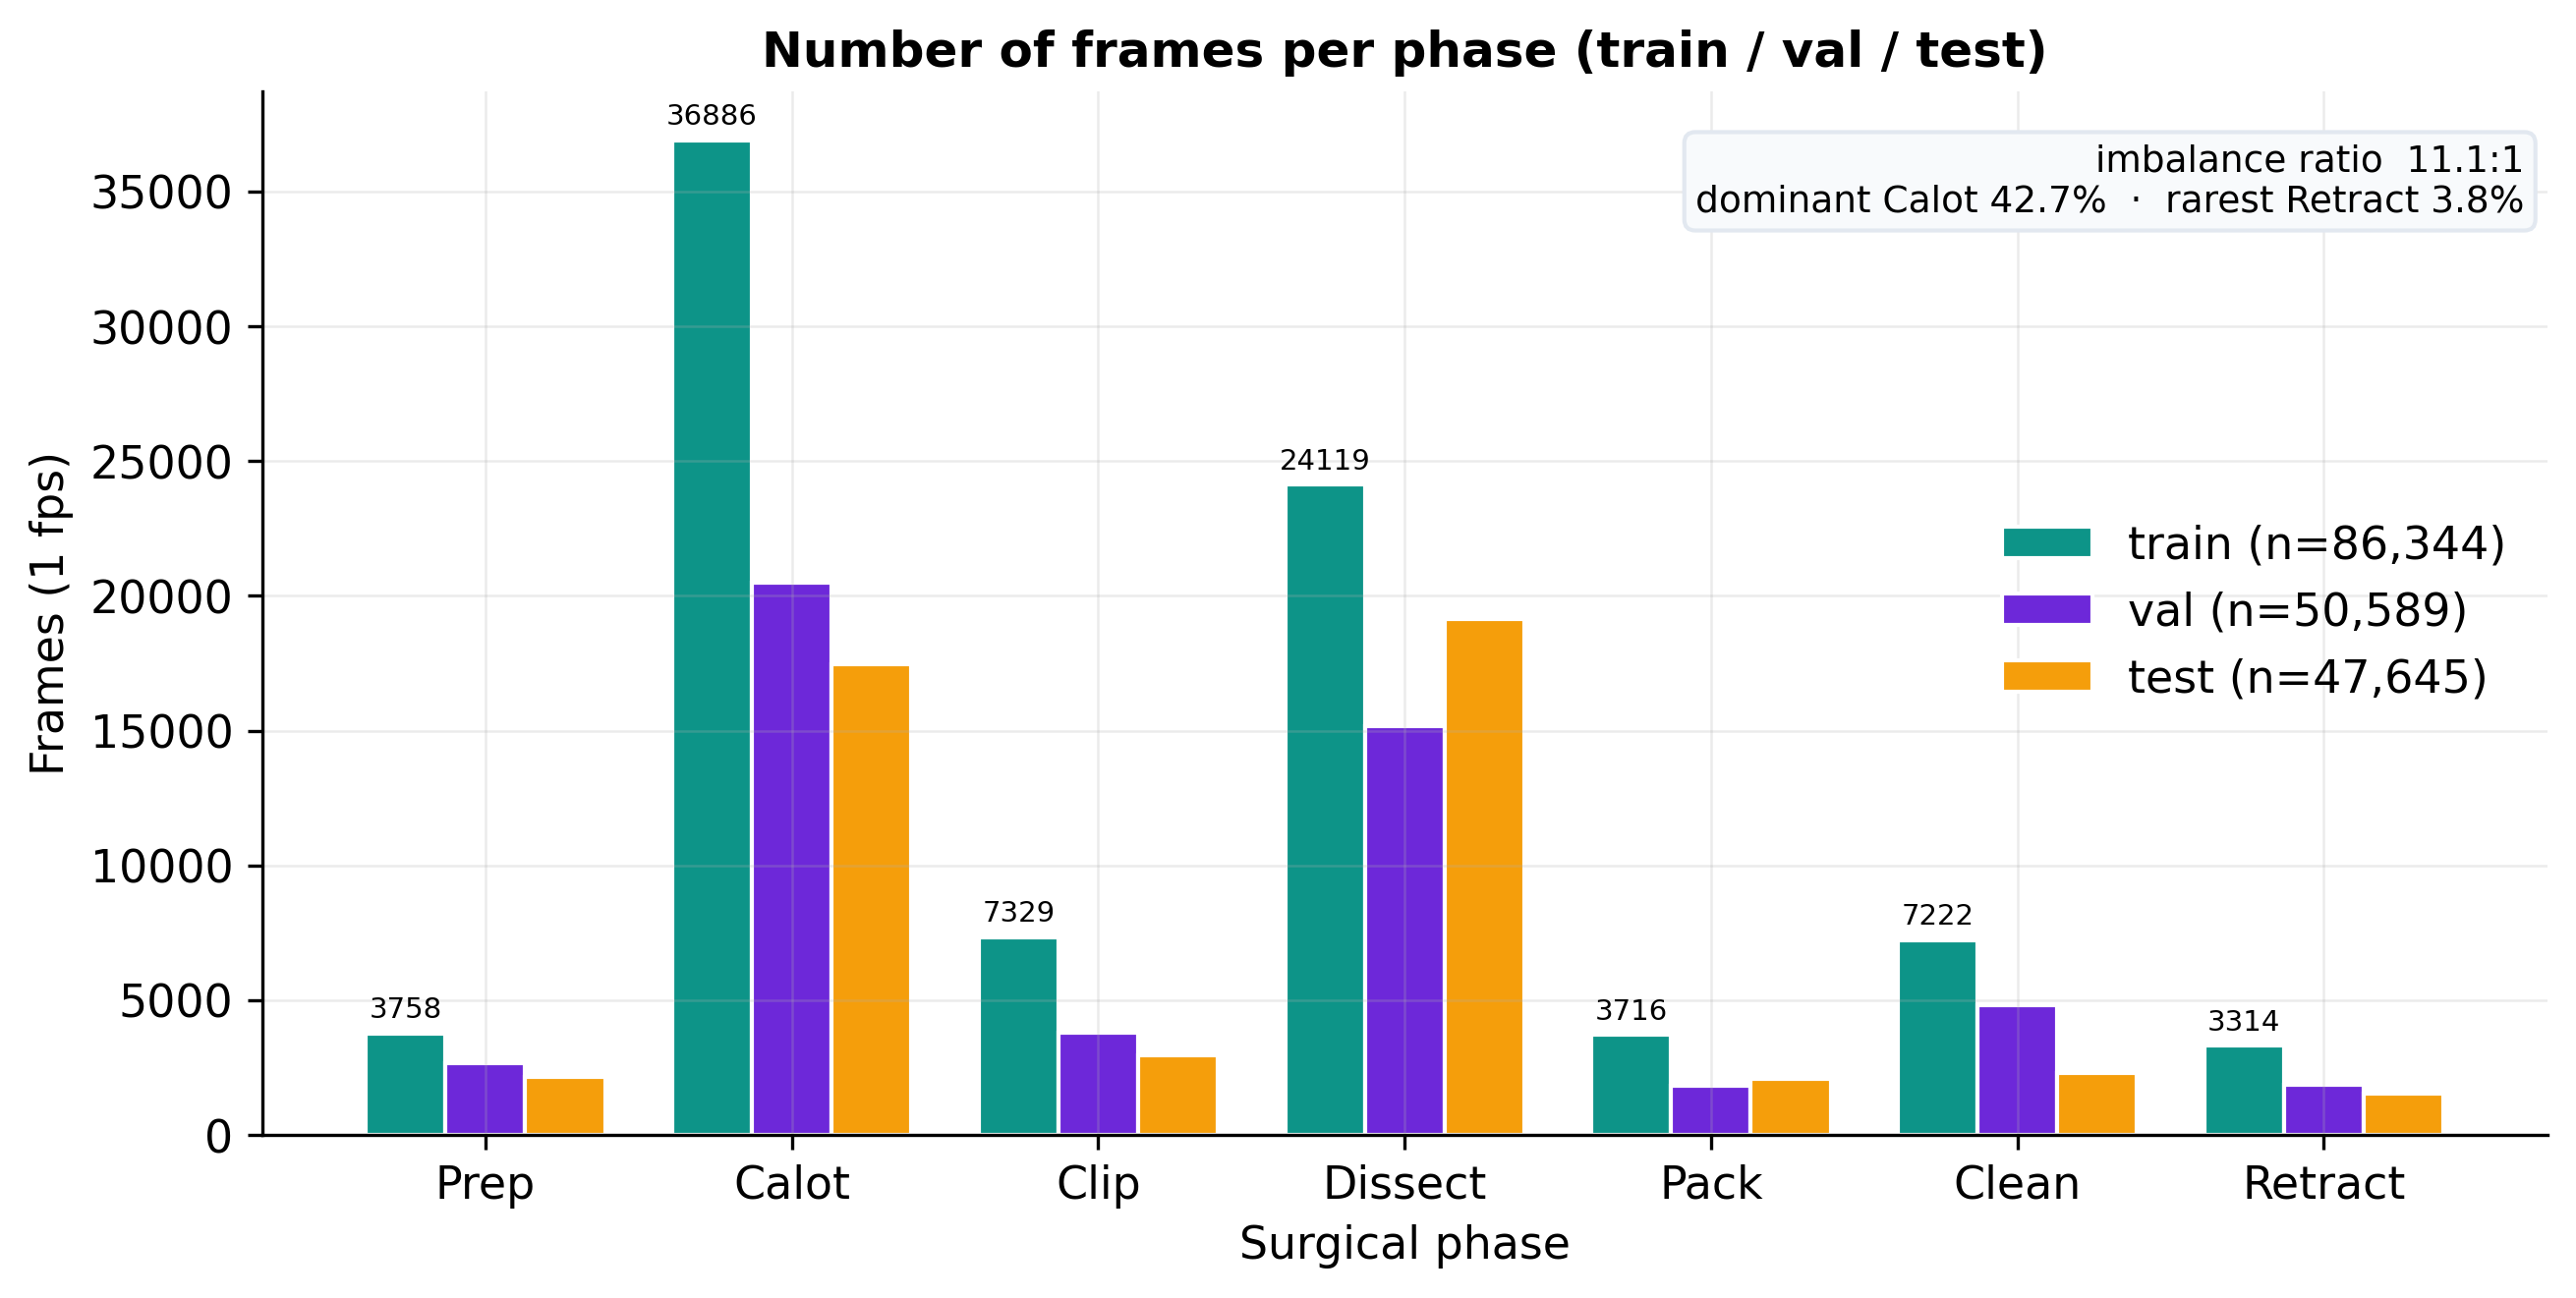
\includegraphics[width=\textwidth]{figures/class_distribution.png}
\caption{Number of frames per phase in the training, validation, and test splits. The common phases (Calot, Dissection) dominate, while the closing phases (Packaging, Retraction) are rare; the proportions are similar across splits.}
\label{fig:class_distribution}
\end{figure}

\section{Model Architectures}

Three architectures are compared, called M1, M2, and M3. All three have the same overall shape, shown in Figure~\ref{fig:transfer_learning}: a backbone turns each of the eight frames into a feature vector, a temporal model reads the sequence of eight vectors, and two small output layers predict, for each frame, the phase and which tools are present. All backbones start from ImageNet-pretrained weights~\cite{deng2009imagenet} loaded through the \texttt{timm} library~\cite{wightman2019timm}.

\begin{figure}[H]
\centering
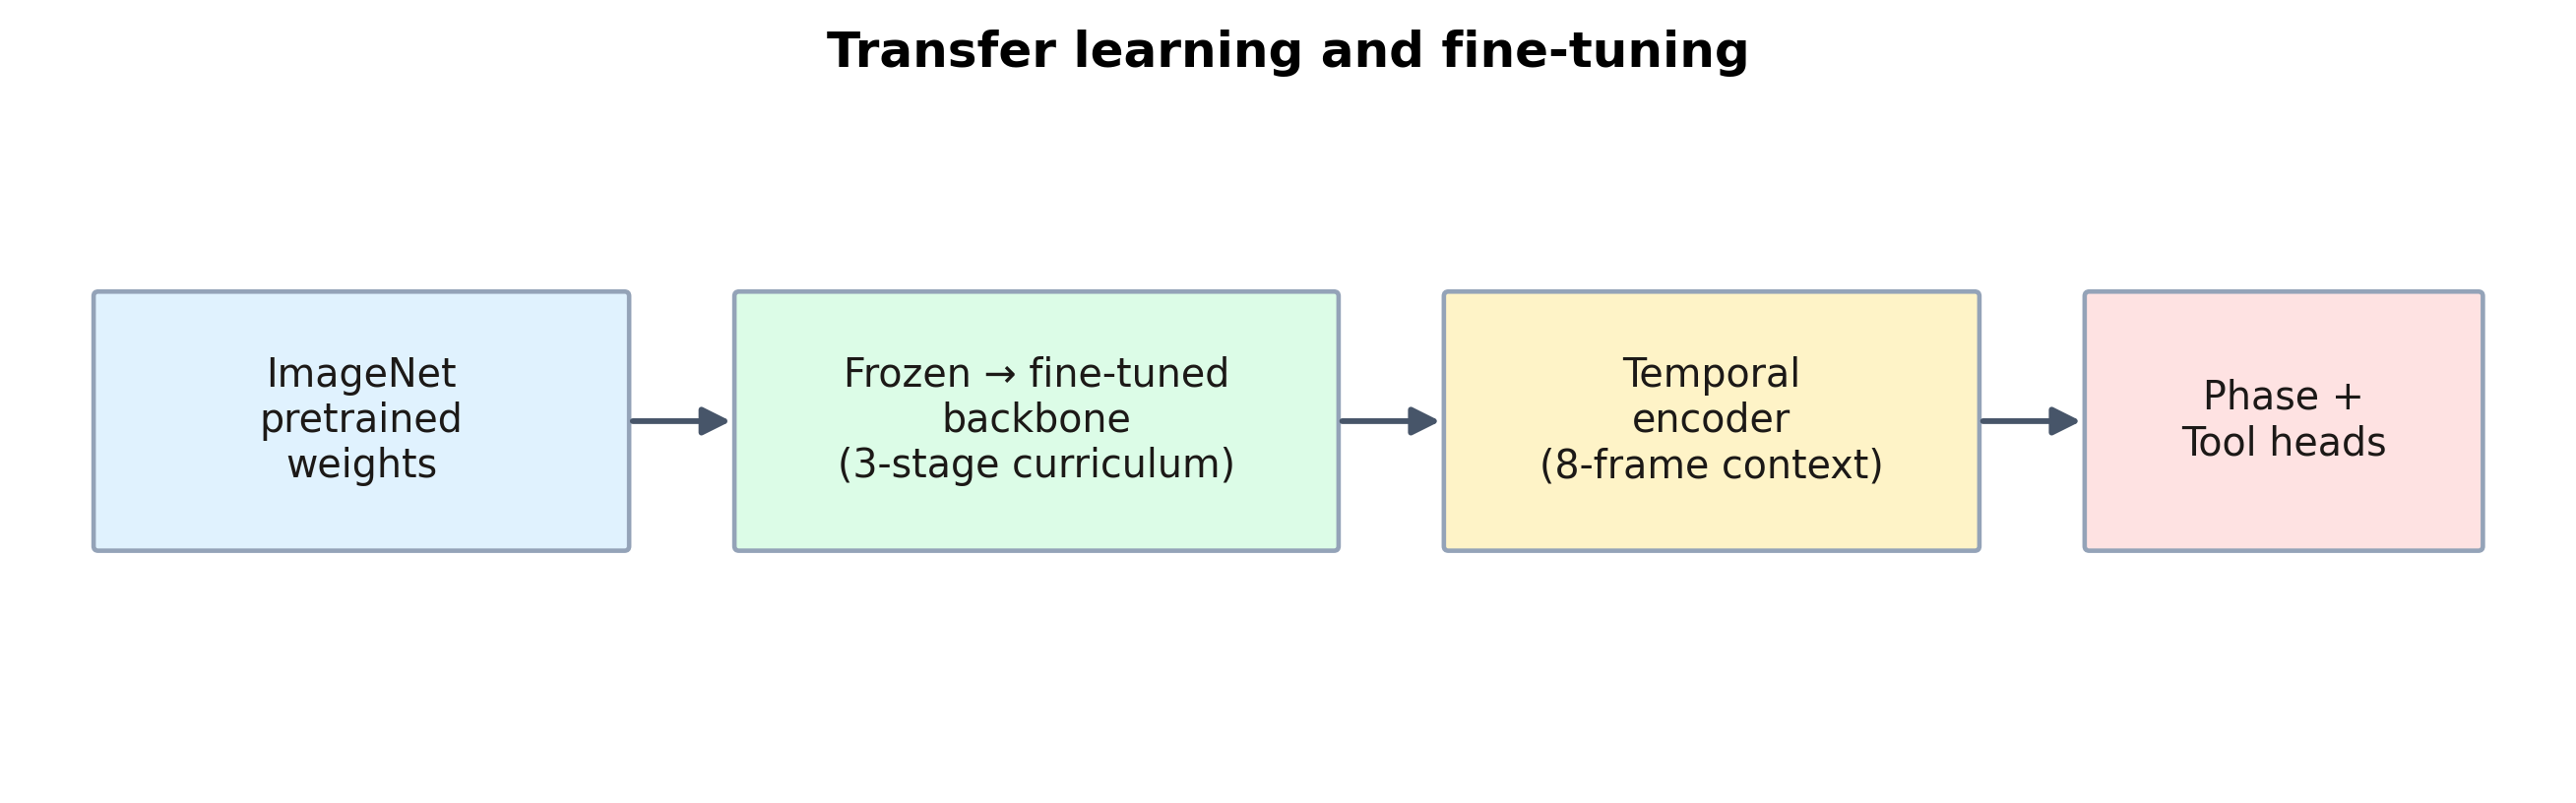
\includegraphics[width=\textwidth]{figures/transfer_learning.png}
\caption{Transfer learning and fine-tuning. The backbone starts from ImageNet weights and is fine-tuned in three stages; an eight-frame temporal model adds context; two output layers predict the phase and the tools.}
\label{fig:transfer_learning}
\end{figure}

\subsection{M1 --- ResNet-50 + Bidirectional LSTM}

The backbone is a ResNet-50~\cite{he2016deep} with ImageNet weights, giving 2048-dimensional features. The temporal model is a two-layer bidirectional LSTM with hidden size 512. Trainable parameters: 35.7~M. This follows SV-RCNet~\cite{jin2018svrcnet}.

\subsection{M2 --- EfficientNet-B3 + Temporal Convolutional Network}

The backbone is EfficientNet-B3~\cite{tan2019efficientnet} (1536-dimensional output). The temporal model is a two-stage temporal convolutional network~\cite{czempiel2020tecno} with eight dilated layers per stage and 64 filters, a smaller version of TeCNO that fits the memory budget. Trainable parameters: 11.2~M.

\subsection{M3 --- Swin-Tiny + Transformer}

The backbone is Swin Transformer-Tiny~\cite{liu2021swin} (768-dimensional output). The temporal model is a three-layer Transformer encoder~\cite{vaswani2017attention} with six heads, model size 384, and feed-forward size 768---kept small on purpose to fit the 4~GB budget. Trainable parameters: 31.6~M.

In all three models, dropout of 0.3 is applied between the temporal model and the output layers. The phase output is one linear layer giving seven scores; the tool output gives seven independent sigmoid values.

\begin{table}[H]
\centering
\caption{Summary of the three evaluated architectures.}
\label{tab:architectures}
\begin{tabular}{lllrl}
\toprule
\textbf{Model} & \textbf{Backbone} & \textbf{Temporal model} & \textbf{Params (M)} & \textbf{Family} \\
\midrule
M1 & ResNet-50      & Bidirectional LSTM  & 35.7 & CNN + RNN \\
M2 & EfficientNet-B3 & Multi-stage TCN     & 11.2 & CNN + TCN \\
M3 & Swin-Tiny      & Transformer encoder & 31.6 & ViT + Attention \\
\bottomrule
\end{tabular}
\end{table}

\section{Training Pipeline}

The training pipeline is designed around the 11:1 imbalance. It tackles the problem in four ways---class weighting, label smoothing, the extra tool task, and a staged schedule---and the ablation study (Section~\ref{sec:ablation}) measures how much each helps. Figure~\ref{fig:training_pipeline} gives an overview.

\begin{figure}[H]
\centering
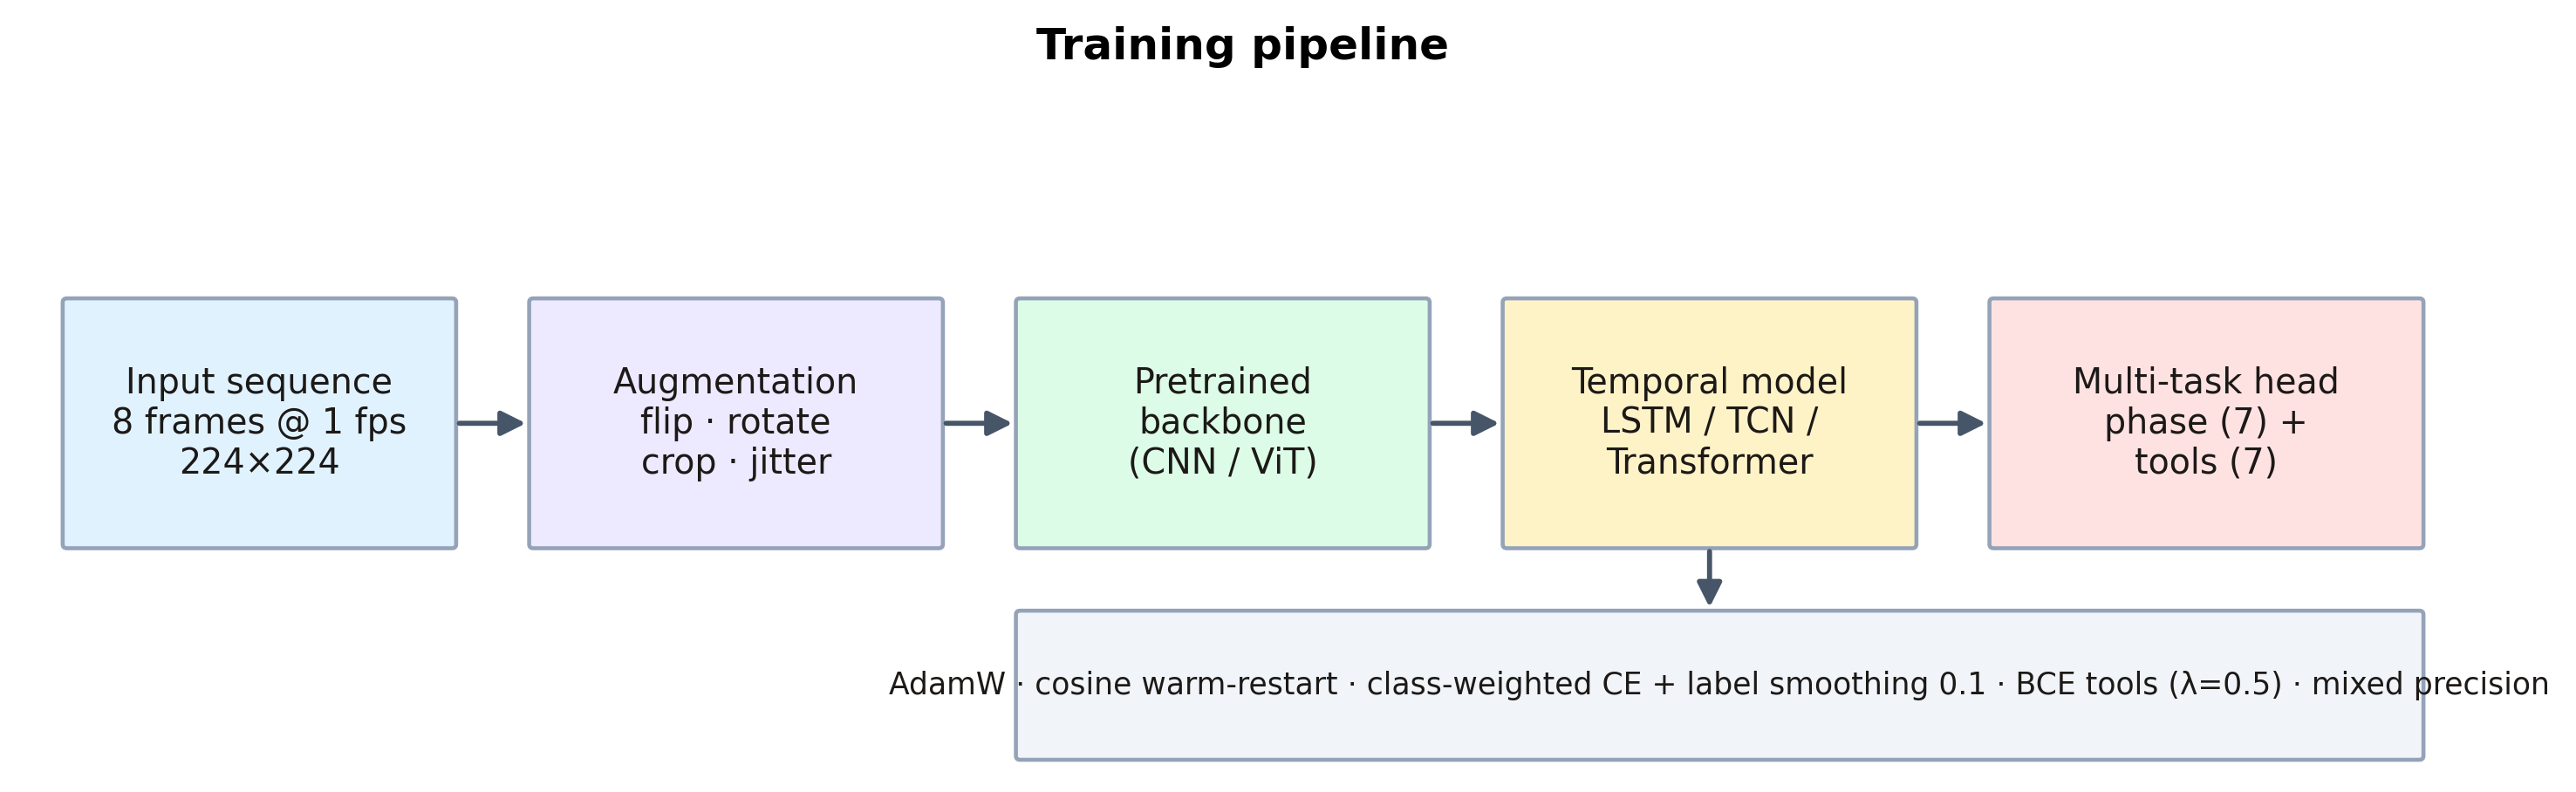
\includegraphics[width=\textwidth]{figures/training_pipeline.png}
\caption{Overview of the training pipeline. An eight-frame sequence is augmented, passed through the backbone and the temporal model, and classified by the output layers. Training uses AdamW with a cosine schedule, class-weighted cross-entropy with label smoothing for the phase, and binary cross-entropy for the tools.}
\label{fig:training_pipeline}
\end{figure}

\subsection{Loss Function}

The total loss is a weighted sum of a phase term and a tool term:
\begin{equation}
\mathcal{L} = \mathcal{L}_{\text{phase}}(z_{\text{phase}}, y_{\text{phase}}) + \lambda \cdot \mathcal{L}_{\text{tool}}(z_{\text{tool}}, y_{\text{tool}})
\label{eq:total_loss}
\end{equation}
where $\mathcal{L}_{\text{phase}}$ is class-weighted cross-entropy with label smoothing 0.1, $\mathcal{L}_{\text{tool}}$ is binary cross-entropy averaged over the seven tools, and $\lambda = 0.5$. Class weights are computed automatically as the inverse class frequency on the training split:
\begin{equation}
w_c = \frac{N}{C \cdot n_c}
\label{eq:class_weight}
\end{equation}
where $N$ is the total number of training frames, $C = 7$ is the number of phases, and $n_c$ is the number of frames in phase $c$. The weights are scaled to sum to the number of classes. This offsets the $11.1\times$ imbalance without ignoring the common phases.

\subsection{Three-Stage Schedule}

Training runs in three stages. In Stage 1 (5 epochs) the backbone is frozen and only the temporal model and output layers are trained. Stage 2 (10 epochs) continues this. In Stage 3 (10 epochs) the backbone is unfrozen and the whole network is fine-tuned, with the backbone learning rate set ten times smaller than the rest. The ablation runs use a shorter $3/6/6$ version.

\subsection{Optimisation}

The optimiser is AdamW~\cite{loshchilov2019decoupled} with a main learning rate of $1\times10^{-4}$, a backbone learning rate of $1\times10^{-5}$, weight decay of $1\times10^{-4}$, and a cosine schedule~\cite{loshchilov2017sgdr}. Mixed-precision (fp16) training~\cite{micikevicius2018mixed} keeps memory within the 4~GB budget; gradients are clipped to a maximum norm of 1.0. The batch sizes are 4 (M1), 8 (M2), and 4 (M3), the largest that fit in memory. Training stops early if validation macro-F1 does not improve for five epochs.

\subsection{Hardware and Software}

All experiments ran on one NVIDIA GeForce RTX 2050 laptop GPU (4~GB) with an Intel Core i7 CPU and 24~GB of RAM, under Windows 11, using Python 3.13, PyTorch 2.6 with CUDA 12.4, torchvision, timm, OpenCV, and scikit-learn.

\section{Evaluation Metrics}

Accuracy alone is misleading on Cholec80: a model that always predicts the two common phases scores well while ignoring the short closing phases. The following metrics are therefore reported alongside accuracy.

\begin{itemize}
    \item \textbf{Macro-F1.} The average of the seven per-phase F1 scores, giving every phase equal weight regardless of how common it is. This is the main metric for choosing models.
    \item \textbf{Per-phase precision / recall / F1.} Shown together with the confusion matrix to see where each model fails.
    \item \textbf{Edit score.} A segment-level metric that judges the quality of the predicted phase \emph{sequence} rather than each frame on its own.
    \item \textbf{Expected Calibration Error (ECE) and Negative Log-Likelihood (NLL).} Used in the calibration analysis (Section~\ref{sec:calibration}).
\end{itemize}

At test time, the predicted phase for each frame is the one with the highest score, and a median filter of length fifteen is run over each video's predictions to remove single-frame errors.

\section{Real-Time Decoding and Calibration}
\label{sec:decoding}

Besides the median filter, this thesis adds a decoder that turns the per-frame scores into a clean phase sequence using only past and present frames, so that it could run during surgery.

\subsection{Temperature Calibration}

For each model a single number $T^\star$ (the temperature) is found on the validation set by minimising the negative log-likelihood over a grid of values. Dividing the scores by $T^\star$ before the softmax tones down over-confident predictions and lowers the ECE, without changing which phase is chosen. The fitted values are 1.3 (M1), 1.1 (M2), and 1.2 (M3)---all above 1.0, which means all three models were over-confident.

\subsection{Learned Transition Table}

A transition table $A$, where $A[i, j]$ is the probability of moving from phase $i$ to phase $j$ from one second to the next, is built from the 40 training videos by counting one-step transitions at 1~fps (with a small smoothing constant). The table is strongly diagonal---the chance of staying in the same phase from one second to the next is between 0.988 and 0.999---and the off-diagonal weight sits on the next phase, matching the fixed order of cholecystectomy.

\subsection{Real-Time Decoder}

The decoder keeps a running score $\alpha_t[c]$ for each phase $c$, equal to the best total score of any path ending in phase $c$ at time $t$. At each step,
\begin{equation}
\alpha_t[c] = \log\,\text{softmax}(z_t / T^\star)[c] + \max_{c'} \big( \alpha_{t-1}[c'] + \log A[c', c] \big),
\label{eq:viterbi}
\end{equation}
and the predicted phase is the one with the highest $\alpha_t$. Each step costs only 49 operations for seven phases, so it runs much faster than real time. The calibrated scores and the transition table are added together in log space; if the scores are too sharp, the table is ignored, which is why calibration is needed for the table to help.

The decoder is compared against three baselines: raw predictions, median-15 smoothing, and an \textbf{offline} pass over the whole video that enforces the fixed phase order using future frames. The offline pass needs the full video, so it is an upper bound, not a method that could run live.

\section{Ablation and Ensemble Design}

Four ablations each change one thing relative to the M1 baseline, to see what that one thing is worth: \textbf{A1} removes the tool-detection task (phase only); \textbf{A2} removes class weighting (plain cross-entropy); \textbf{A3} doubles the sequence to sixteen frames and halves the batch size; and \textbf{A4} turns off the median filter at test time.

Three ways of combining the three models are tested: \textbf{simple averaging} of their predictions, \textbf{averaging weighted by validation F1}, and \textbf{majority voting} over their per-frame choices. All three pass through the same median filter before evaluation. The weighted average is
\begin{equation}
\hat{y} = \arg\max_c \sum_{m=1}^{M} \omega_m \, p_m(c \mid x),
\label{eq:ensemble}
\end{equation}
where $M = 3$ is the number of models, $p_m(c \mid x)$ is the probability model $m$ gives to phase $c$, and the weight $\omega_m$ is proportional to model $m$'s validation macro-F1.

% ======================= CHAPTER 4: EXPERIMENTS AND RESULTS ==========================
\chapter{Experiments and Results}

All experiments were run on the single 4~GB GPU described in Section~3.3, with the random seed fixed at 42. Results are reported on the held-out test set of twenty videos (IDs 61--80), which no model saw during training or model selection.

\section{Comparison of the Three Models}

\subsection{Overall Results}

Table~\ref{tab:model_comparison} reports accuracy and macro-F1 for the three models, before and after median smoothing.

\begin{table}[H]
\centering
\caption{Test-set results for the three models. Best values in \textbf{bold}.}
\label{tab:model_comparison}
\begin{tabular}{lcccc}
\toprule
\textbf{Model} & \textbf{Raw Acc.} & \textbf{Raw Macro-F1} & \textbf{Smoothed Acc.} & \textbf{Smoothed Macro-F1} \\
\midrule
M1 --- ResNet-50 + BiLSTM      & 0.832 & 0.775 & 0.837 & 0.781 \\
M2 --- EfficientNet-B3 + TCN   & 0.818 & 0.739 & 0.824 & 0.748 \\
\textbf{M3 --- Swin-Tiny + Transformer} & \textbf{0.857} & \textbf{0.807} & \textbf{0.862} & \textbf{0.815} \\
\bottomrule
\end{tabular}
\end{table}

The Swin-Transformer M3 is best on every metric, with a smoothed macro-F1 of \textbf{0.815}---3.4 points above the ResNet-LSTM and 6.7 points above the EfficientNet-TCN. Its accuracy of 0.862 is in the same range as Trans-SVNet~\cite{gao2021transsvnet} on this dataset, even though it was trained on a single 4~GB laptop GPU. Figure~\ref{fig:arch_compare} plots each model's score against its number of parameters: M3 wins without being the largest model, and M1 has more parameters yet scores lower, so model size is not what limits the result here.

\begin{figure}[H]
\centering
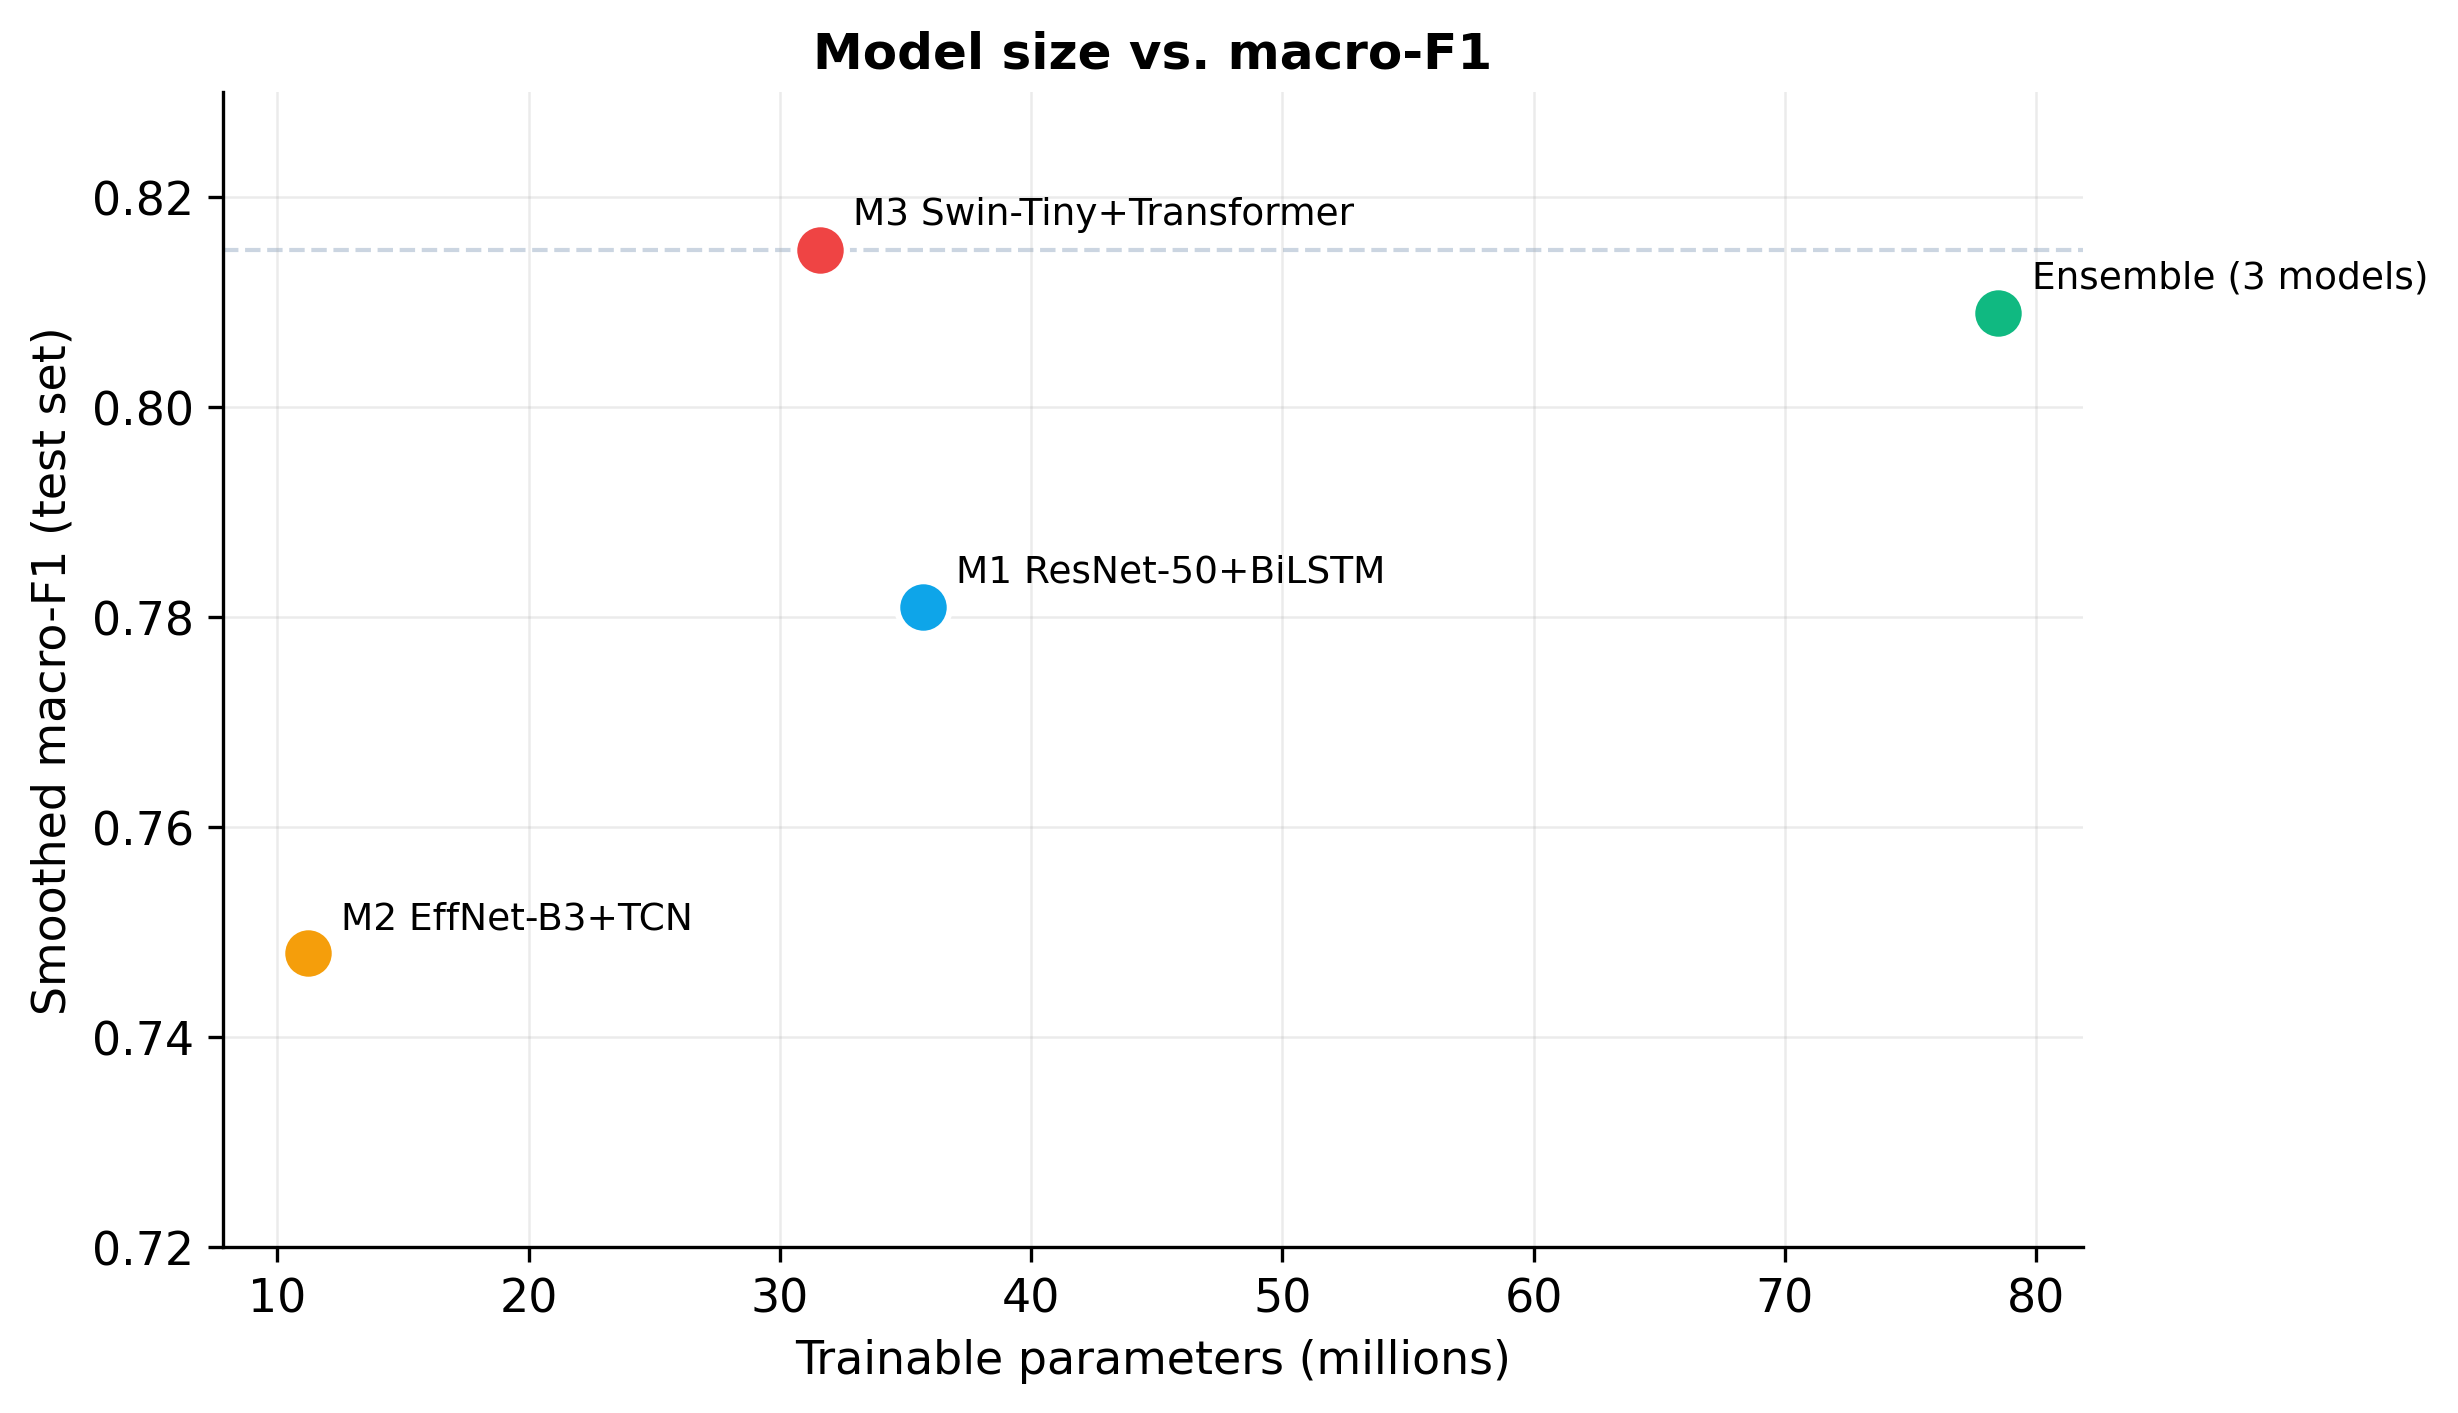
\includegraphics[width=\figwidth]{figures/arch_compare.png}
\caption{Model size versus macro-F1. The Swin-Transformer (M3) scores highest without being the largest; the EfficientNet-TCN (M2) is the smallest and the weakest, partly because its Stage-3 fine-tuning was cut short by limited memory.}
\label{fig:arch_compare}
\end{figure}

\subsection{Training Dynamics}

Figure~\ref{fig:training_history} shows the loss and accuracy curves for the three models over the three stages. M1 and M3 train smoothly, and their validation accuracy jumps once the backbone is unfrozen in Stage 3. M2's curve is shorter: with the EfficientNet-B3 backbone unfrozen, memory use reached about 97\% of the 4~GB limit and only part of Stage 3 finished, so M2's numbers are a lower bound on what it could reach with more memory.

\begin{figure}[H]
\centering
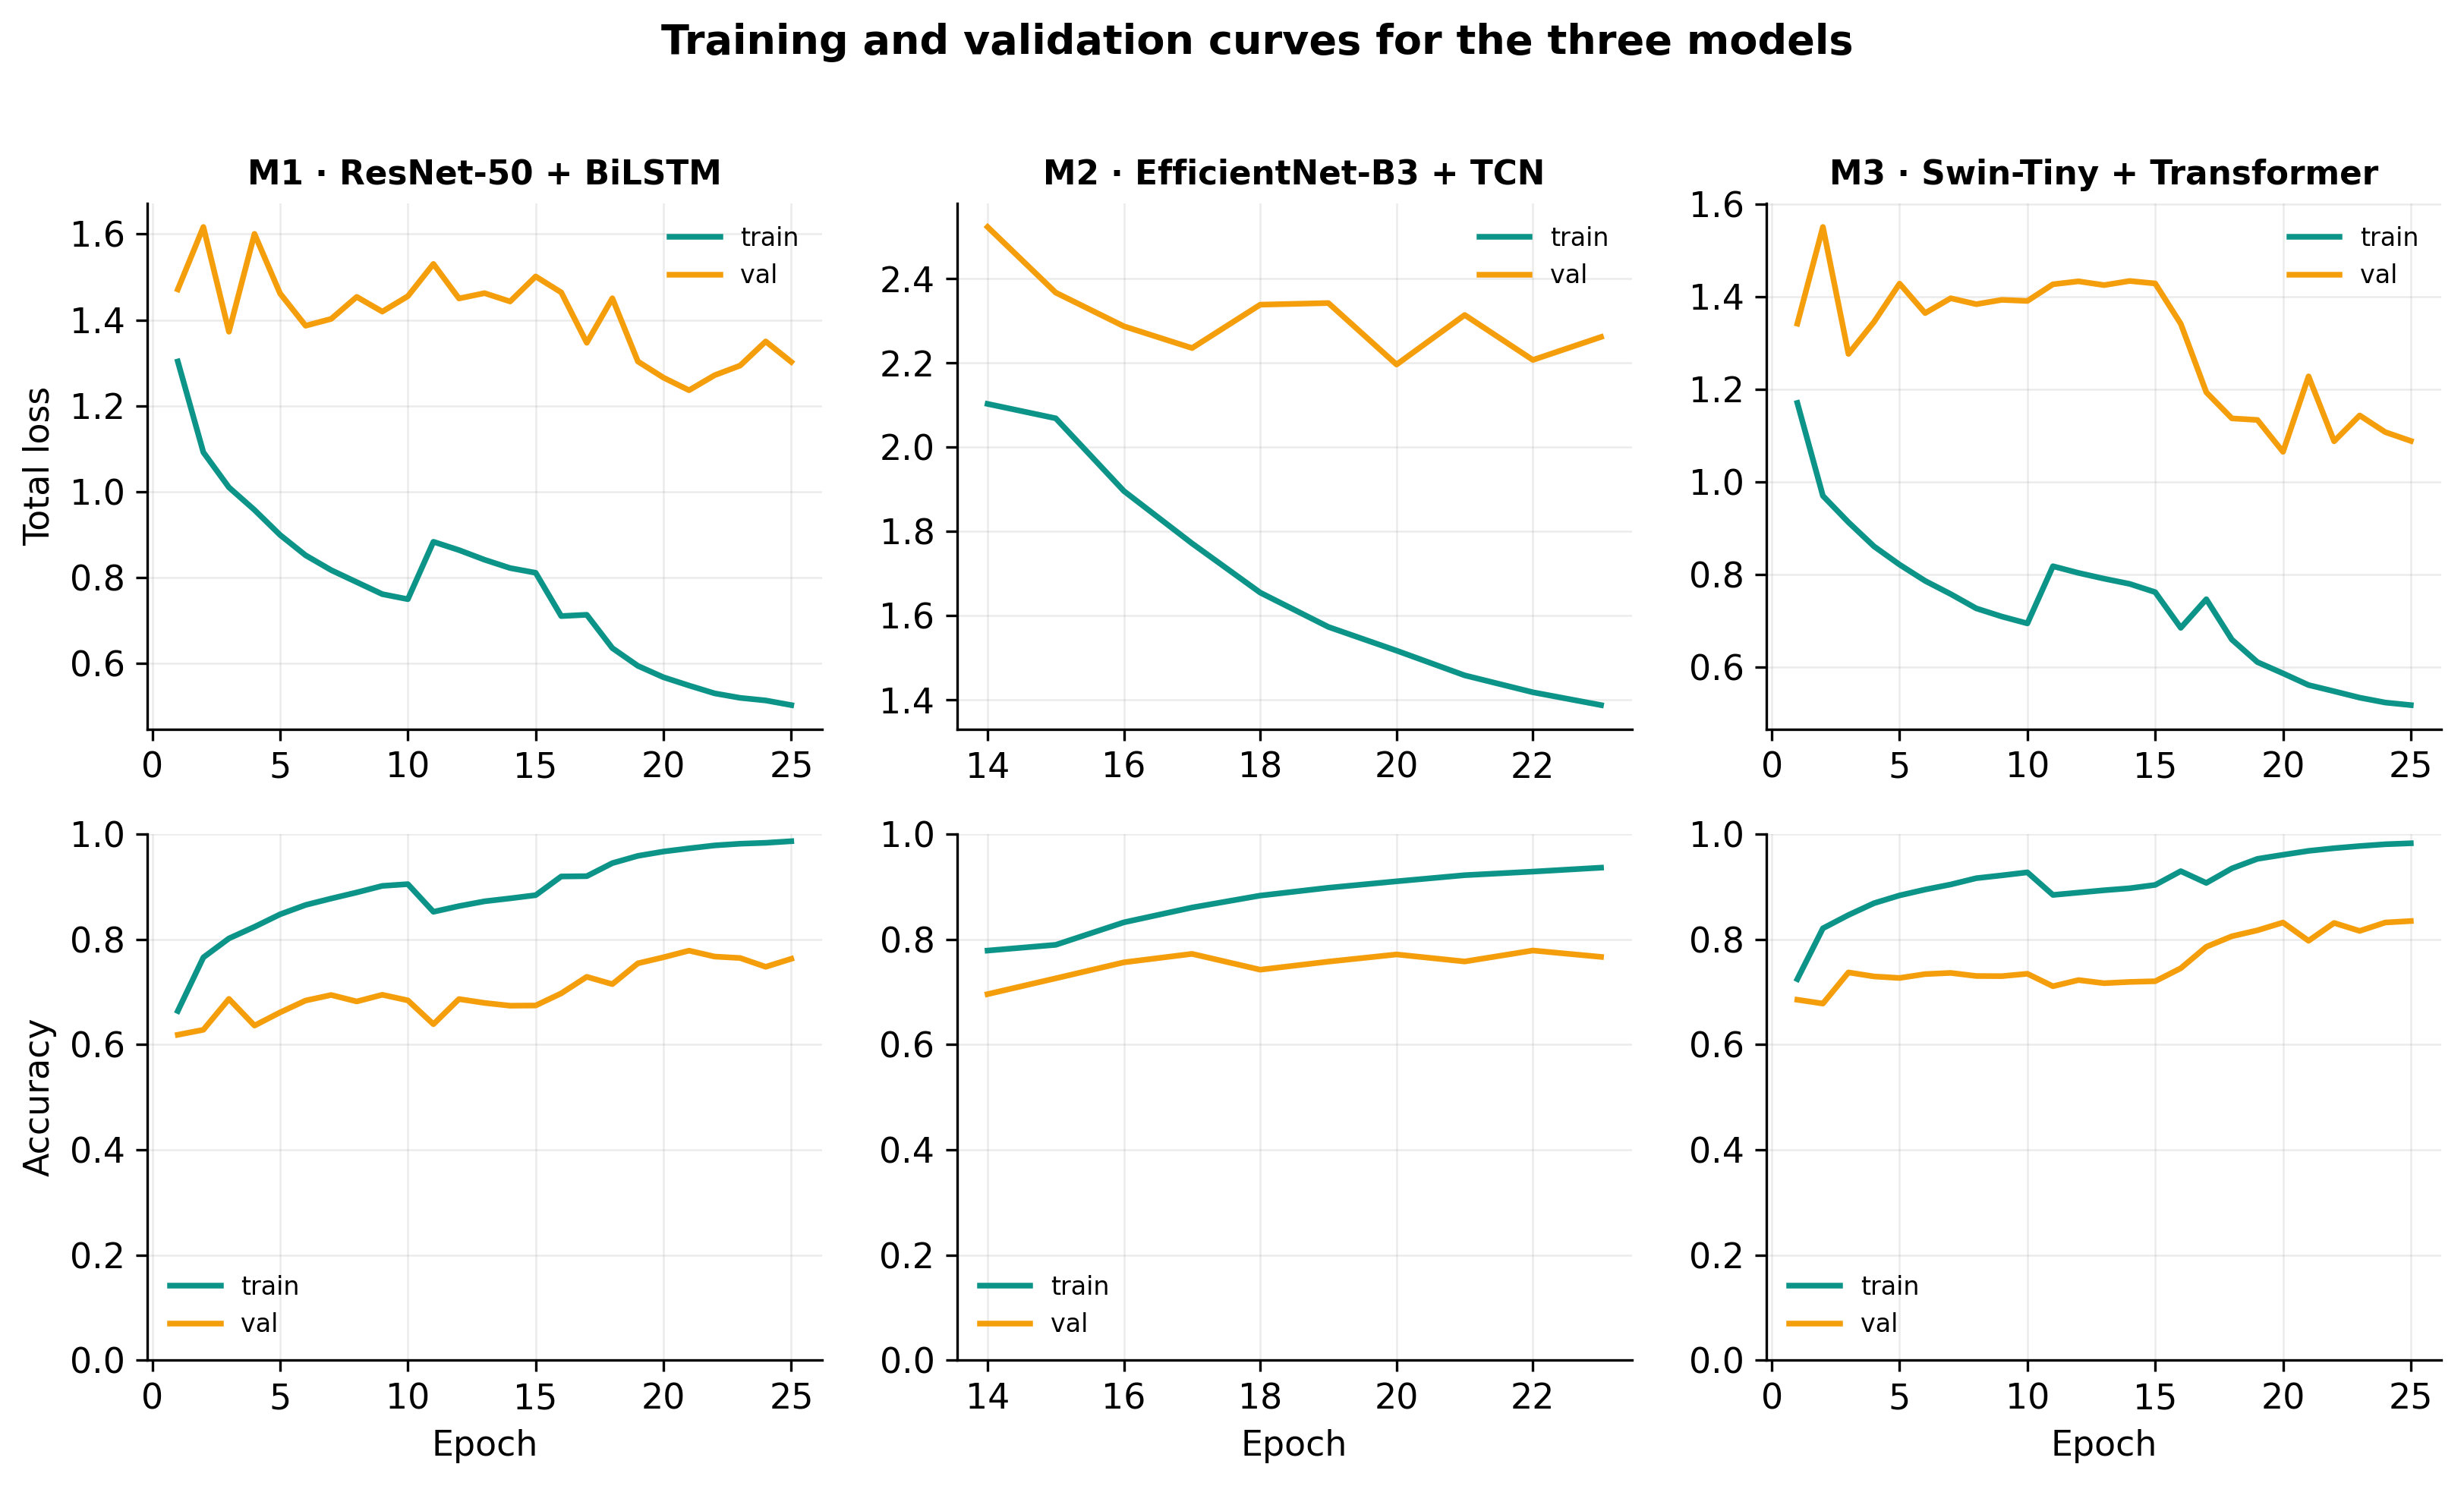
\includegraphics[width=\textwidth]{figures/train_history.png}
\caption{Training and validation loss and accuracy over epochs for the three models. M3 shows the clearest jump in Stage 3; M2's run is cut short by limited memory during backbone fine-tuning.}
\label{fig:training_history}
\end{figure}

\subsection{Per-Phase Analysis}

Table~\ref{tab:per_class_m3} details per-class precision, recall, and F1 for M3 on the raw test predictions.

\begin{table}[H]
\centering
\caption{Per-phase precision, recall, and F1 for M3 (raw predictions, test set). The weakest phase is in \textbf{bold}.}
\label{tab:per_class_m3}
\begin{tabular}{lccc}
\toprule
\textbf{Phase} & \textbf{Precision} & \textbf{Recall} & \textbf{F1} \\
\midrule
Preparation               & 0.830 & 0.803 & 0.816 \\
Calot triangle dissection & 0.880 & 0.895 & 0.887 \\
Clipping and cutting      & 0.815 & 0.796 & 0.806 \\
Gallbladder dissection    & 0.868 & 0.885 & 0.877 \\
Gallbladder packaging     & 0.881 & 0.759 & 0.816 \\
Cleaning and coagulation  & 0.741 & 0.663 & \textbf{0.700} \\
Gallbladder retraction    & 0.727 & 0.764 & 0.745 \\
\bottomrule
\end{tabular}
\end{table}

The two common phases have the highest F1, as expected. The weakest is Cleaning and coagulation (recall 0.663): the model often mistakes cleaning for the surrounding dissection phase, which also shows up in the confusion matrix (Figure~\ref{fig:confusion_m3}). Importantly, all seven phases are above F1 $=0.70$, so the class-weighted loss does prevent the model from collapsing onto the common phases.

\begin{figure}[H]
\centering
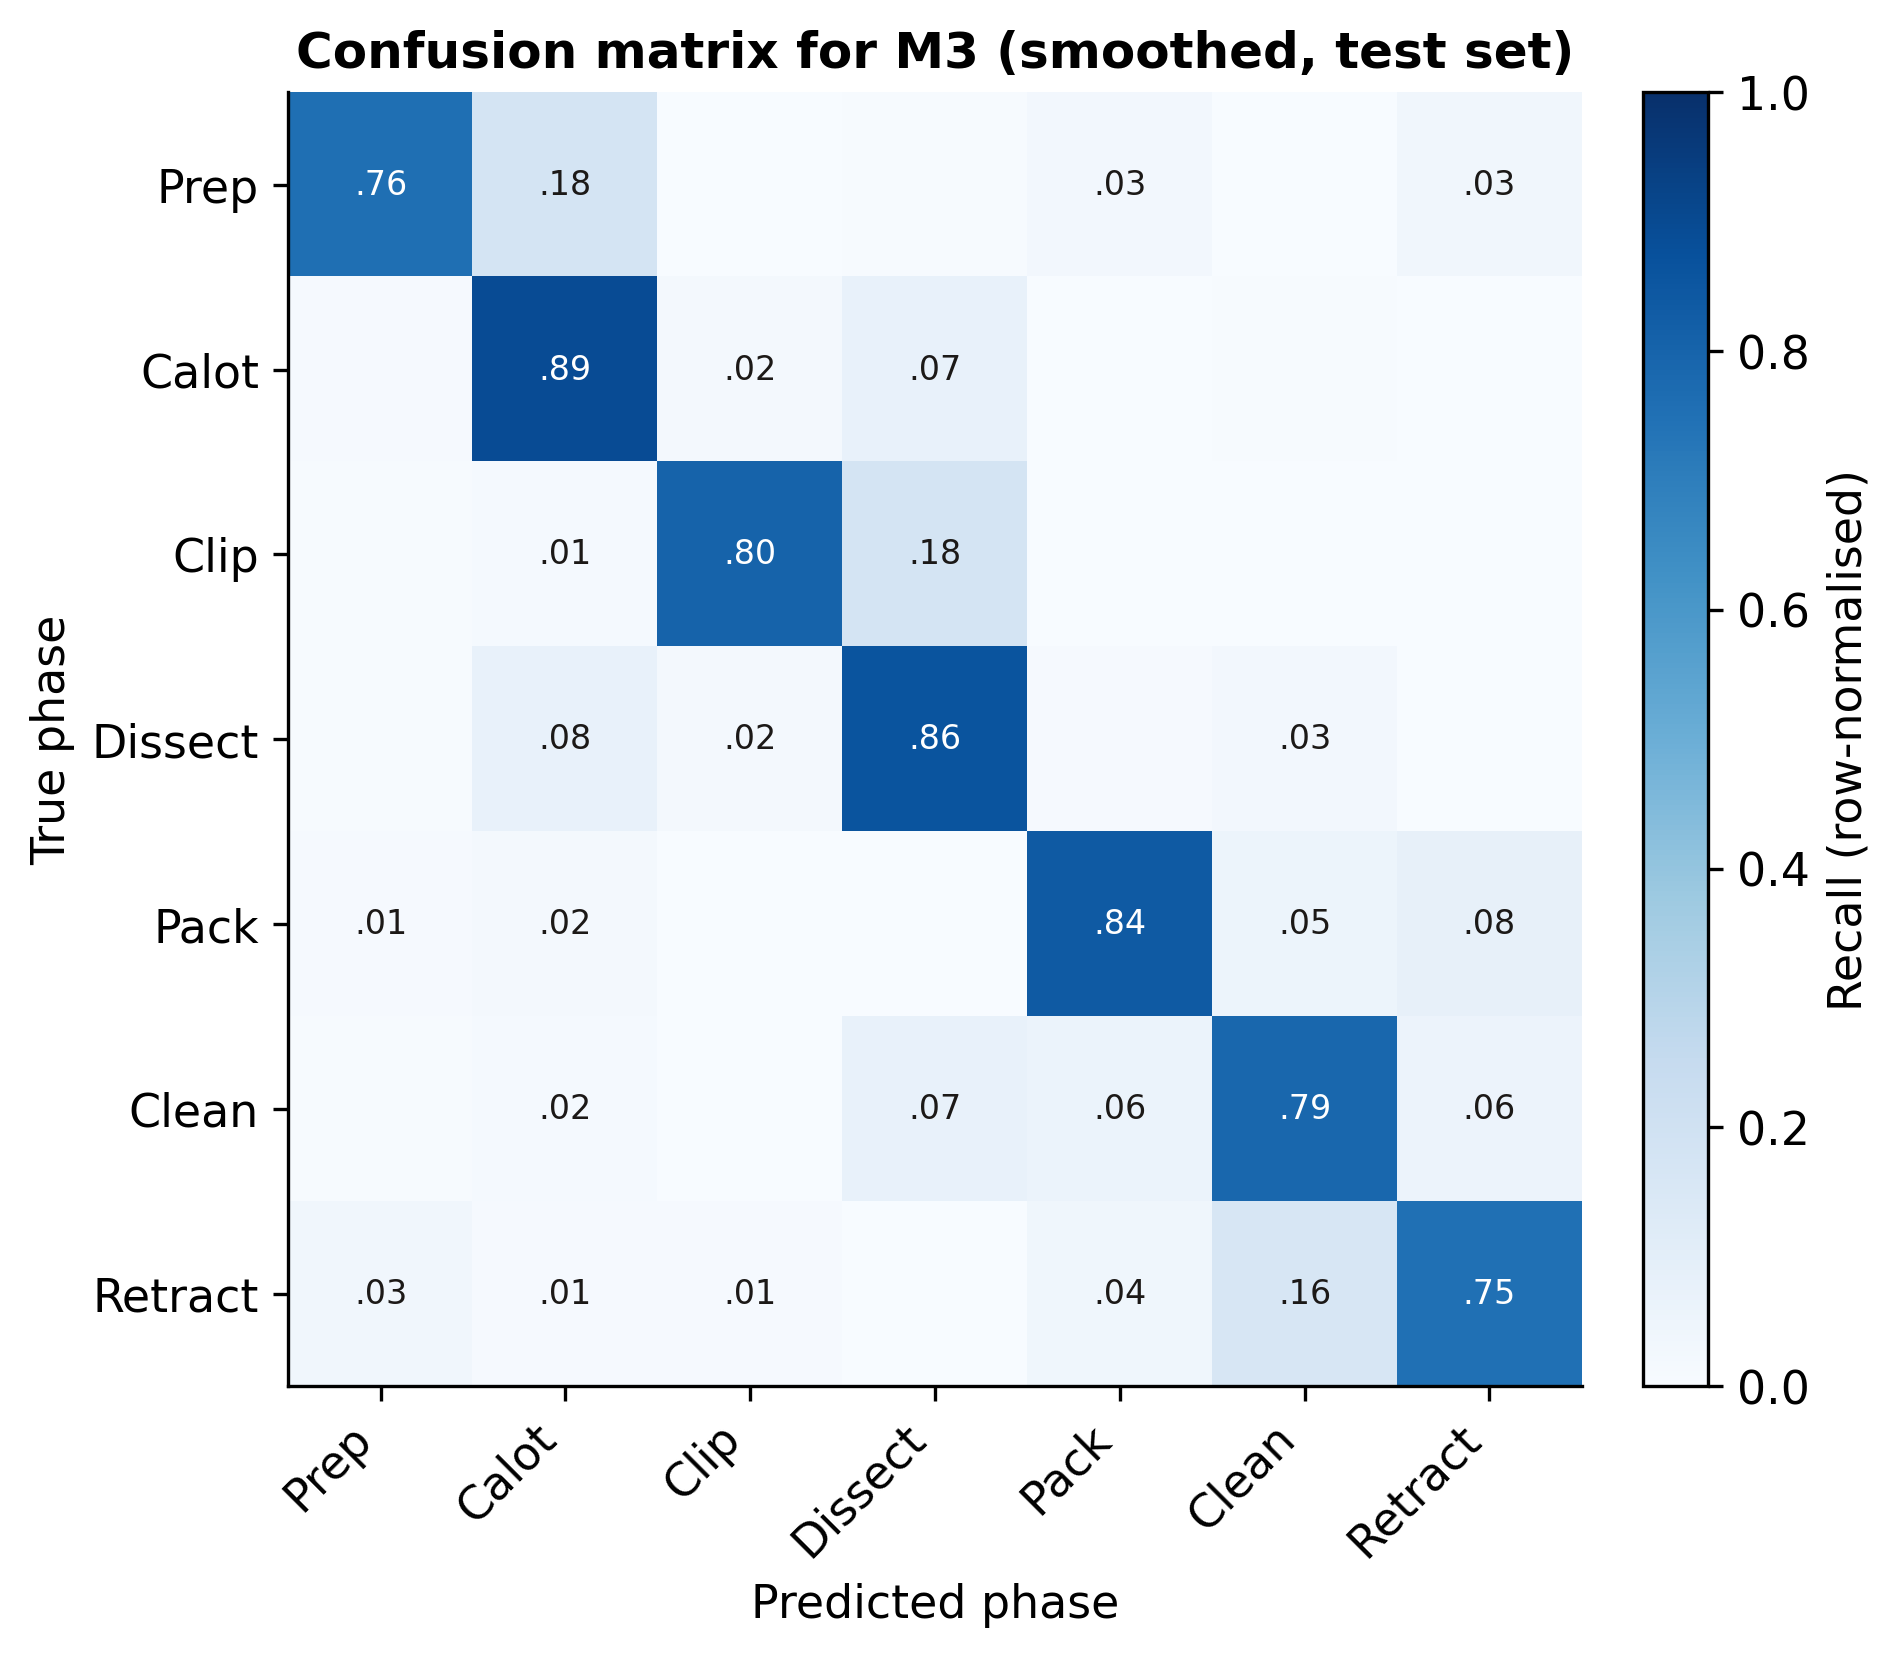
\includegraphics[width=\figwidth]{figures/confusion_m3.png}
\caption{Confusion matrix (each row adds to 1) for M3 on the smoothed test predictions. The main mistakes are Cleaning and Clipping predicted as Dissection---neighbouring phases that look similar---and no phase collapses onto the common ones.}
\label{fig:confusion_m3}
\end{figure}

\section{Ablation Study}
\label{sec:ablation}

Table~\ref{tab:ablation} reports the four ablations against the M1 baseline, all trained with the same optimiser and three-stage schedule.

\begin{table}[H]
\centering
\caption{Ablation study (test-set smoothed macro-F1, change relative to M1).}
\label{tab:ablation}
\begin{tabular}{llcc}
\toprule
\textbf{ID} & \textbf{Modification} & \textbf{Smoothed Macro-F1} & \textbf{$\Delta$F1 vs M1}\\
\midrule
\textbf{M1 baseline} & full configuration & \textbf{0.781} & --- \\
\midrule
A1 & remove tool detection (single-task) & 0.765 & $-1.6\%$ \\
A2 & remove class weighting              & 0.761 & $-2.0\%$ \\
A3 & sequence length 16 instead of 8     & 0.787 & $+0.6\%$ \\
A4 & disable median smoothing            & 0.775 & $-0.6\%$ \\
\bottomrule
\end{tabular}
\end{table}

Three points stand out. First, removing the tool task (A1) costs 1.6 points of macro-F1, confirming that the extra task helps, as EndoNet first noted~\cite{twinanda2017endonet}. Second, removing class weighting (A2) costs 2.0 points, but the loss is uneven: the two rarest phases---Gallbladder retraction and packaging---drop 5.1 and 2.8 points of per-phase F1, while the common Calot phase actually gains 0.7. This is exactly the problem class weighting is meant to fix. Third, A4 shows what the median filter does: it barely changes macro-F1 ($+0.6\%$) but improves the edit score by about 35\%, so its main job is cleaning up the phase sequence, not improving per-frame accuracy. Doubling the sequence length (A3) gives only $+0.6\%$, which means the eight-second window already covers most of the useful context.

Together, class weighting and the tool task are worth almost four points of macro-F1---about the same as the 3.4-point gap between the best and worst architecture. This is the main evidence that, on Cholec80, the training recipe matters as much as the backbone.

\section{Ensemble Results}

Table~\ref{tab:ensemble} compares the three ways of combining the models.

\begin{table}[H]
\centering
\caption{Combining the three models (smoothed, test set). Best values in \textbf{bold}.}
\label{tab:ensemble}
\begin{tabular}{lcc}
\toprule
\textbf{Strategy} & \textbf{Accuracy} & \textbf{Macro-F1} \\
\midrule
M3 alone (best single model)              & 0.856 & 0.799 \\
Ensemble --- simple softmax average       & 0.863 & 0.808 \\
\textbf{Ensemble --- val-F1-weighted average} & \textbf{0.864} & \textbf{0.809} \\
Ensemble --- majority voting              & 0.857 & 0.799 \\
\bottomrule
\end{tabular}
\end{table}

The F1-weighted average beats the best single model by 1.0 point of macro-F1, with M3 getting the largest weight (0.355), then M1 (0.327) and M2 (0.318). The weights are almost equal, which suggests the three models are each capable but make similar mistakes---they tend to be wrong on the same hard frames (usually near phase changes) rather than on different ones. This is why the next section turns to decoding and calibration: if the remaining errors are concentrated and structured, a better decoder may help more than adding more models.

\section{Real-Time Decoding and Calibration}
\label{sec:calibration}

This section compares the real-time decoder of Section~\ref{sec:decoding} with the baselines, using the same per-frame scores for every method so that any difference comes only from the decoding step.

\subsection{Calibration}

Table~\ref{tab:calibration} reports validation ECE and NLL before and after temperature scaling. M1, the most over-confident model, gains the most---its ECE drops by 66\%. For all three models the best temperature is above 1.0, the sign of over-confidence. Figure~\ref{fig:reliability} shows the reliability diagrams: the raw accuracy sits below the diagonal in the high-confidence bins, and temperature scaling pulls the curve back toward the diagonal.

\begin{table}[H]
\centering
\caption{Validation calibration before and after temperature scaling. Best ECE in \textbf{bold}.}
\label{tab:calibration}
\begin{tabular}{lccccc}
\toprule
\textbf{Model} & \textbf{$T^\star$} & \textbf{ECE raw} & \textbf{ECE cal} & \textbf{NLL raw} & \textbf{NLL cal} \\
\midrule
M1 --- ResNet-LSTM      & 1.30 & 0.109 & \textbf{0.037} & 0.897 & 0.855 \\
M2 --- EffNet-TCN       & 1.10 & 0.059 & 0.074 & 0.824 & 0.817 \\
M3 --- Swin-Transformer & 1.20 & 0.074 & 0.070 & 0.688 & 0.667 \\
\bottomrule
\end{tabular}
\end{table}

\begin{figure}[H]
\centering
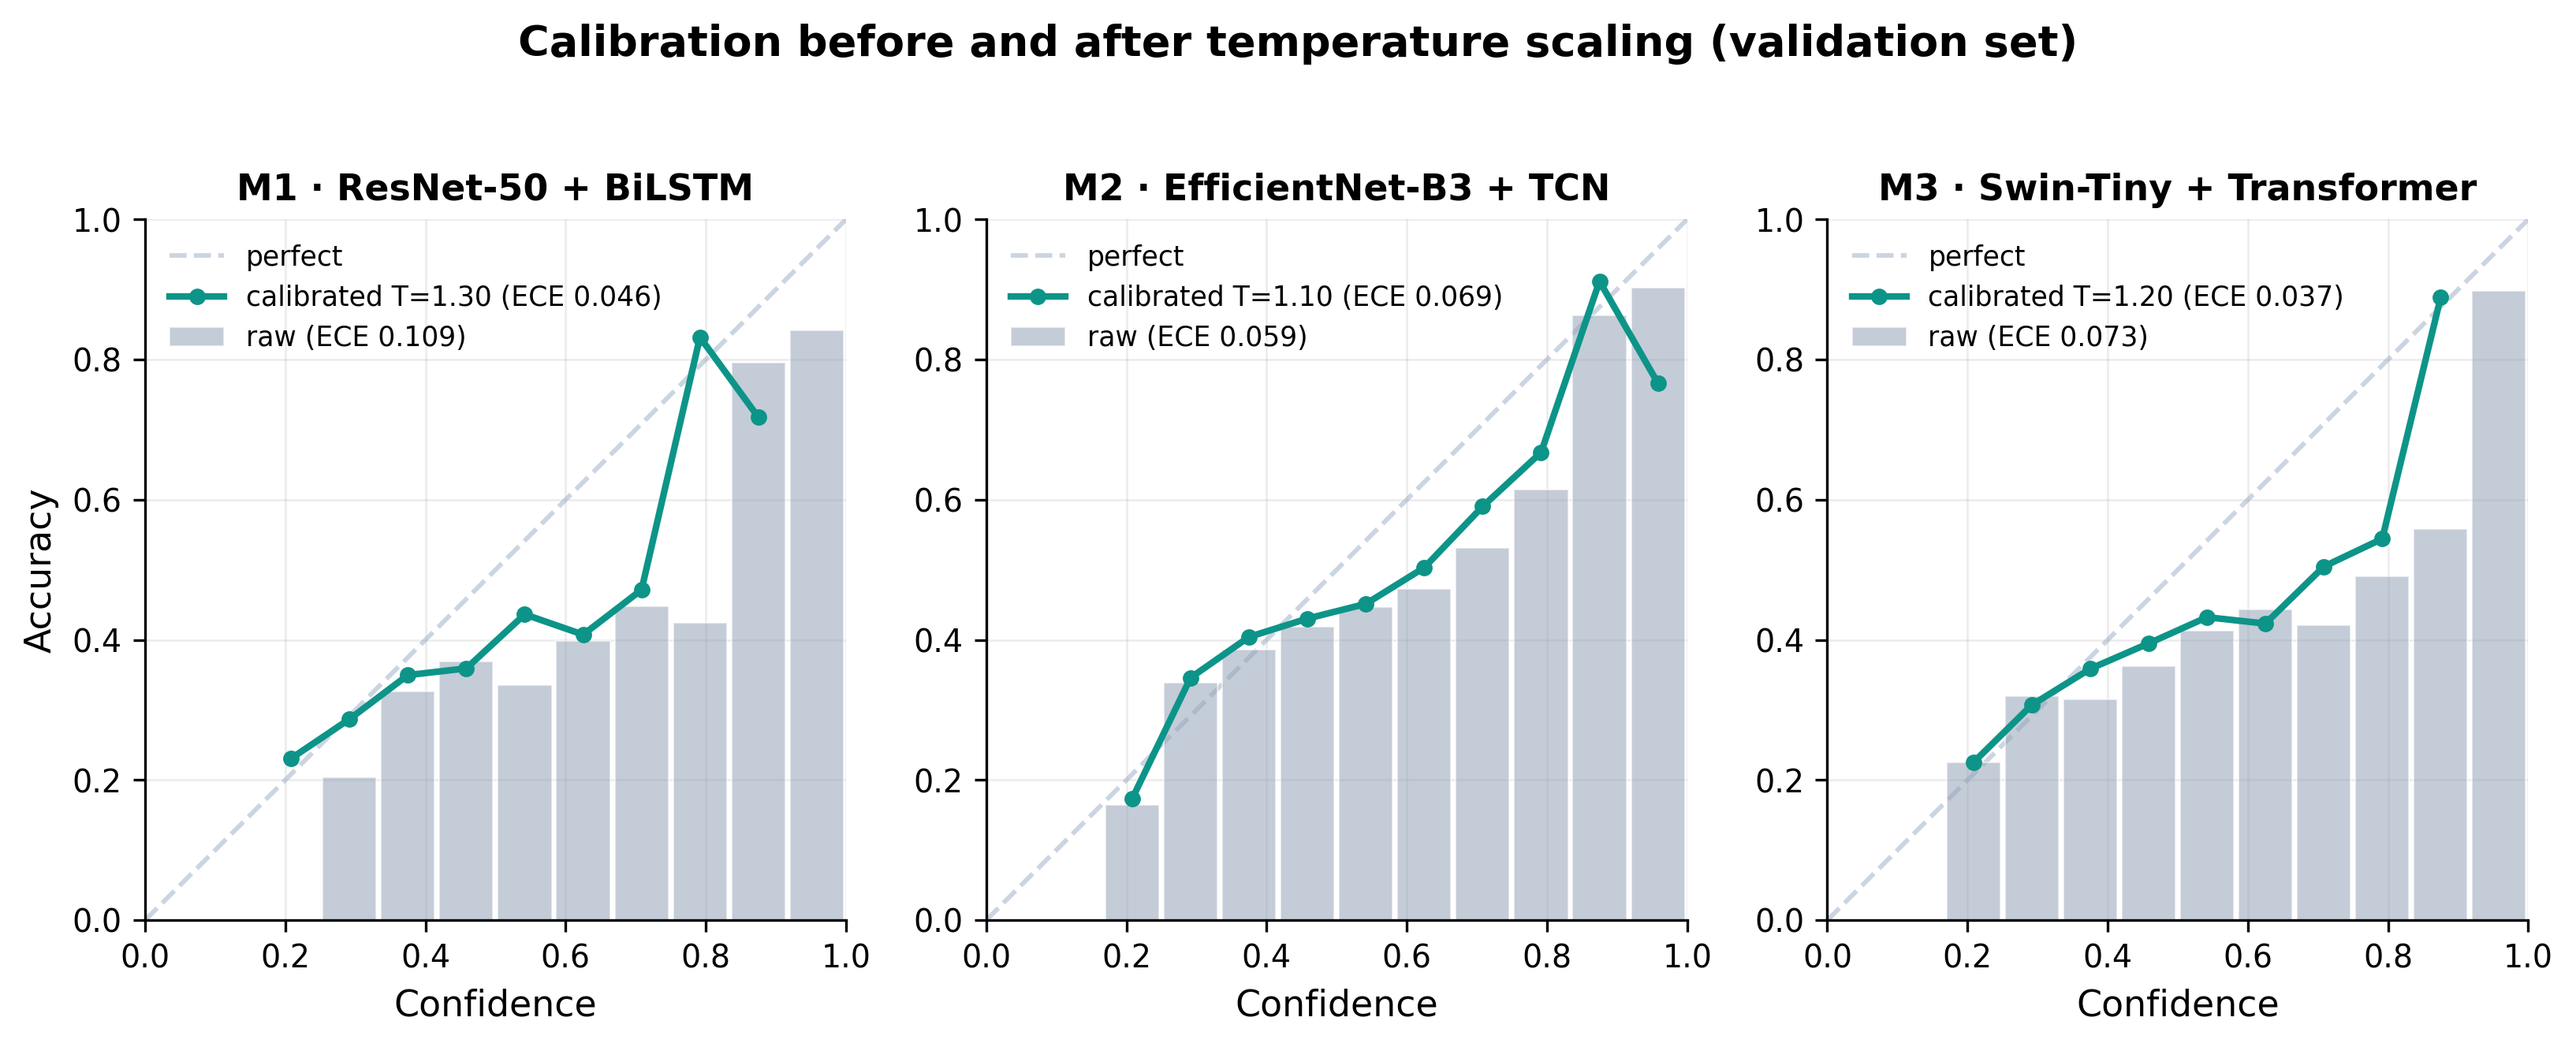
\includegraphics[width=\textwidth]{figures/reliability.png}
\caption{Reliability diagrams on the validation set. Grey bars are the raw accuracy in each confidence bin; the teal curve is after temperature scaling; the dashed diagonal is perfect calibration. M1 moves the most toward the diagonal.}
\label{fig:reliability}
\end{figure}

\subsection{Decoder Benchmark}

Table~\ref{tab:decoder} reports test accuracy and macro-F1 for each decoder on each model. The proposed decoder (calibrated scores plus the transition table) is the best real-time decoder on all three models; the offline decoder is shown only as an upper bound. Figure~\ref{fig:benchmark} shows the same comparison.

\begin{table}[H]
\centering
\caption{Decoder comparison (test set, accuracy / macro-F1). The offline decoder $\dagger$ uses future frames and is only an upper bound. Best \emph{real-time} values in \textbf{bold}.}
\label{tab:decoder}
\begin{tabular}{lccc}
\toprule
\textbf{Decoder} & \textbf{M1 Acc / F1} & \textbf{M2 Acc / F1} & \textbf{M3 Acc / F1} \\
\midrule
Raw predictions          & 82.4 / 0.763 & 81.2 / 0.738 & 85.3 / 0.794 \\
Median-15 filter         & 82.7 / 0.768 & 81.7 / 0.746 & 85.5 / 0.800 \\
Fixed-order + cal        & 82.5 / 0.777 & 82.4 / 0.767 & 86.0 / 0.802 \\
\textbf{Proposed decoder} & \textbf{83.0 / 0.771} & \textbf{82.9 / 0.764} & \textbf{86.0 / 0.806} \\
\midrule
Offline (full video) $\dagger$ & 91.8 / 0.859 & 91.8 / 0.849 & 90.1 / 0.832 \\
\bottomrule
\end{tabular}
\end{table}

\begin{figure}[H]
\centering
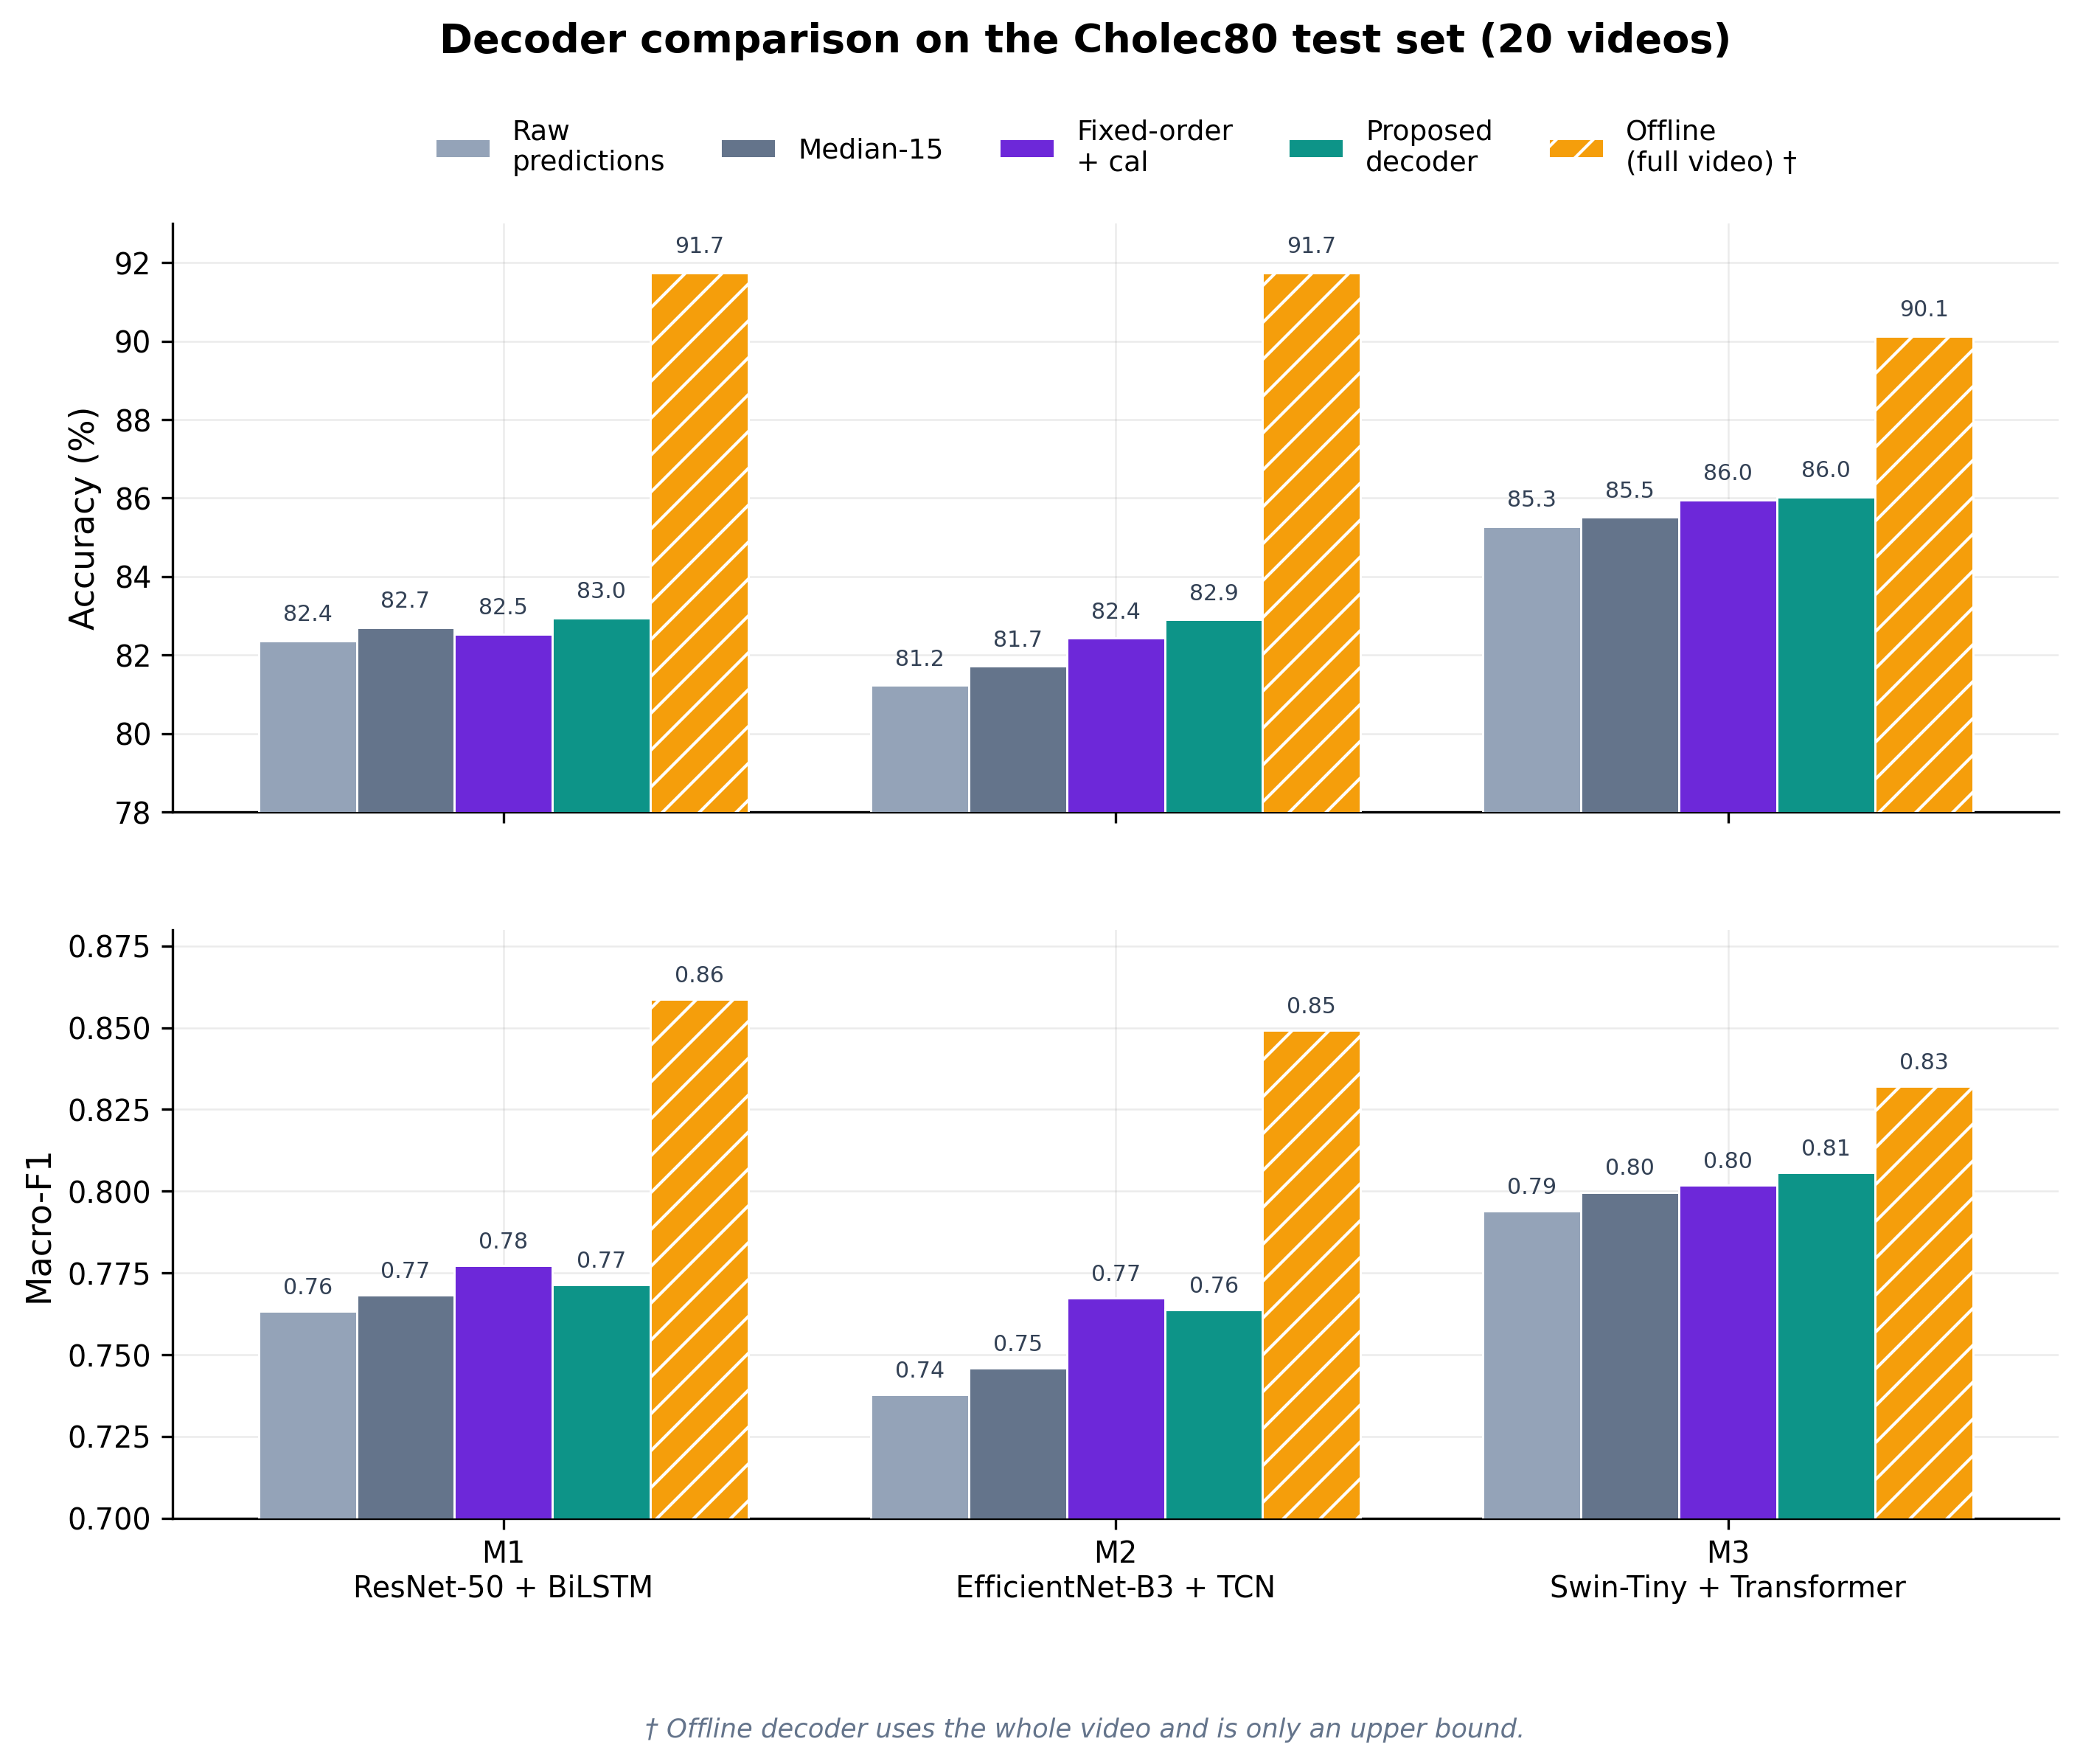
\includegraphics[width=\textwidth]{figures/benchmark.png}
\caption{Decoder comparison on the test set: accuracy and macro-F1. The proposed decoder (teal) is the best real-time option on every model; the offline decoder (amber, hatched) uses future frames and is the upper bound.}
\label{fig:benchmark}
\end{figure}

\subsection{Statistical Significance}

Because the average gains look small, a per-video test is important. Table~\ref{tab:significance} reports a paired Wilcoxon signed-rank test and Cohen's $d$ over the twenty test videos, comparing the proposed decoder with the raw predictions. All three models show a clear, consistent improvement ($p < 0.001$, $d > 0.97$): the gain is small in size but holds across videos rather than being driven by a few outliers. The decoder takes 0.011--0.024~ms per frame, far below the 40~ms available between frames in 25~fps video. Figure~\ref{fig:transition_significance} shows the learned transition table and the per-video gains side by side.

\begin{table}[H]
\centering
\caption{Per-video improvement of the proposed decoder over the raw predictions (20 test videos).}
\label{tab:significance}
\begin{tabular}{lccc}
\toprule
\textbf{Model} & \textbf{$\Delta$Acc (pp)} & \textbf{Wilcoxon $p$} & \textbf{Cohen's $d$} \\
\midrule
M1 --- ResNet-LSTM      & $+0.62$ & $<0.0001$ & 1.38 \\
M2 --- EffNet-TCN       & $+1.74$ & $0.0001$  & 1.25 \\
M3 --- Swin-Transformer & $+0.76$ & $0.0001$  & 0.98 \\
\bottomrule
\end{tabular}
\end{table}

\begin{figure}[H]
\centering
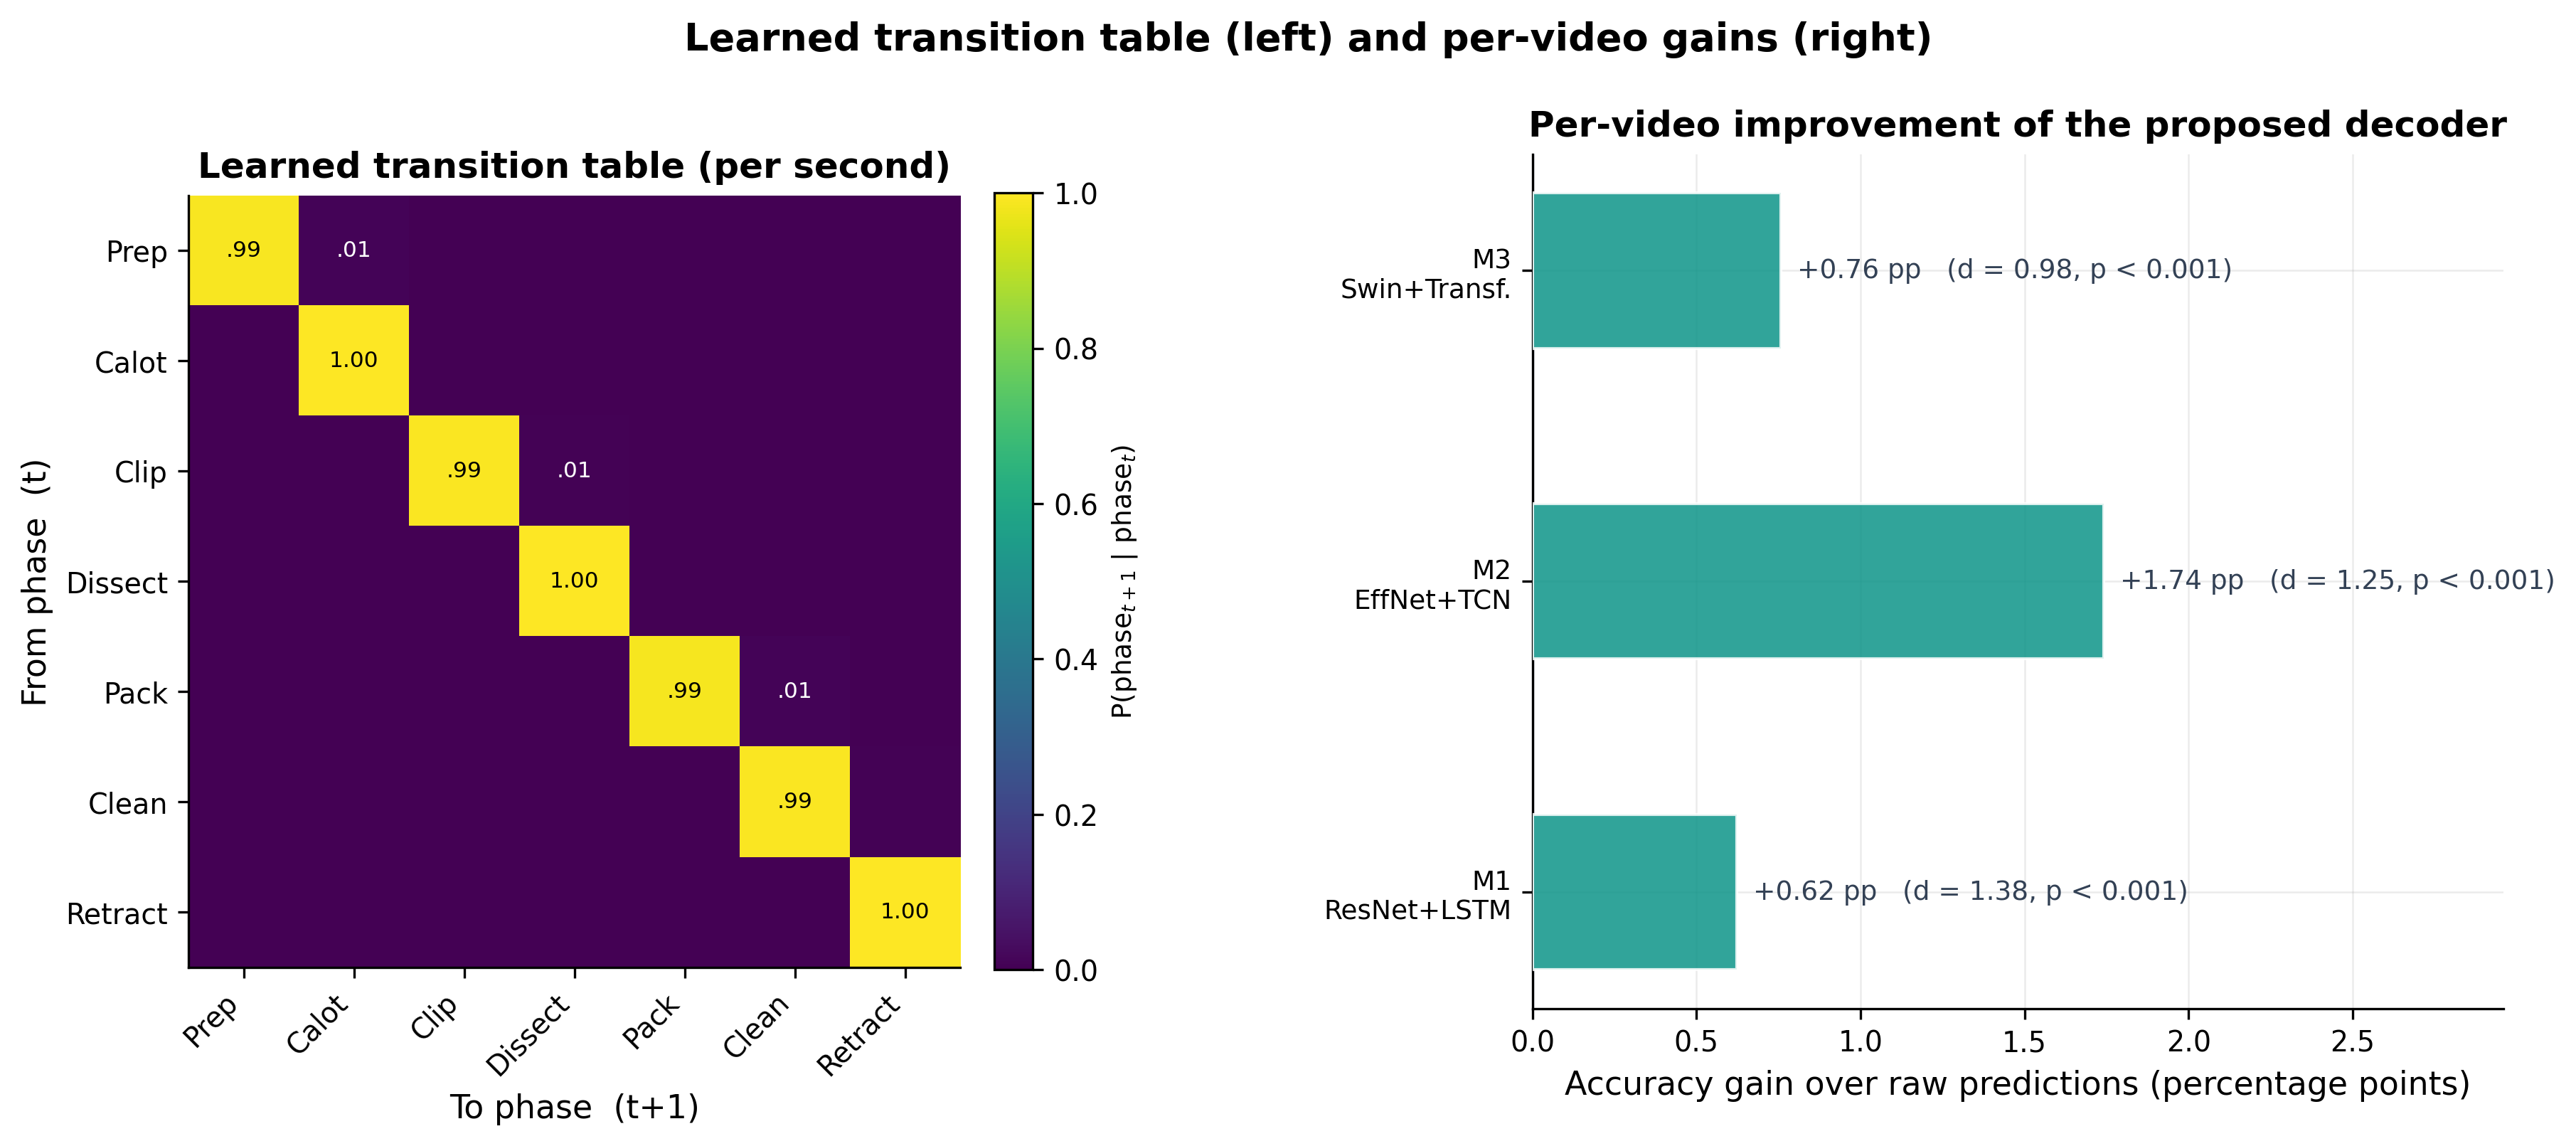
\includegraphics[width=\textwidth]{figures/transition_significance.png}
\caption{Left: the learned per-second transition table, strongly diagonal with the remaining weight on the next phase, matching the fixed phase order. Right: per-video accuracy gain of the proposed decoder over the raw predictions, with Cohen's $d$ and the Wilcoxon $p$-value.}
\label{fig:transition_significance}
\end{figure}

\subsection{Qualitative Example}

Figure~\ref{fig:timeline} shows the predicted phase timeline for one test video. The raw predictions flip back and forth, especially early on; the proposed decoder removes most of these flips and follows the ground truth much more closely.

\begin{figure}[H]
\centering
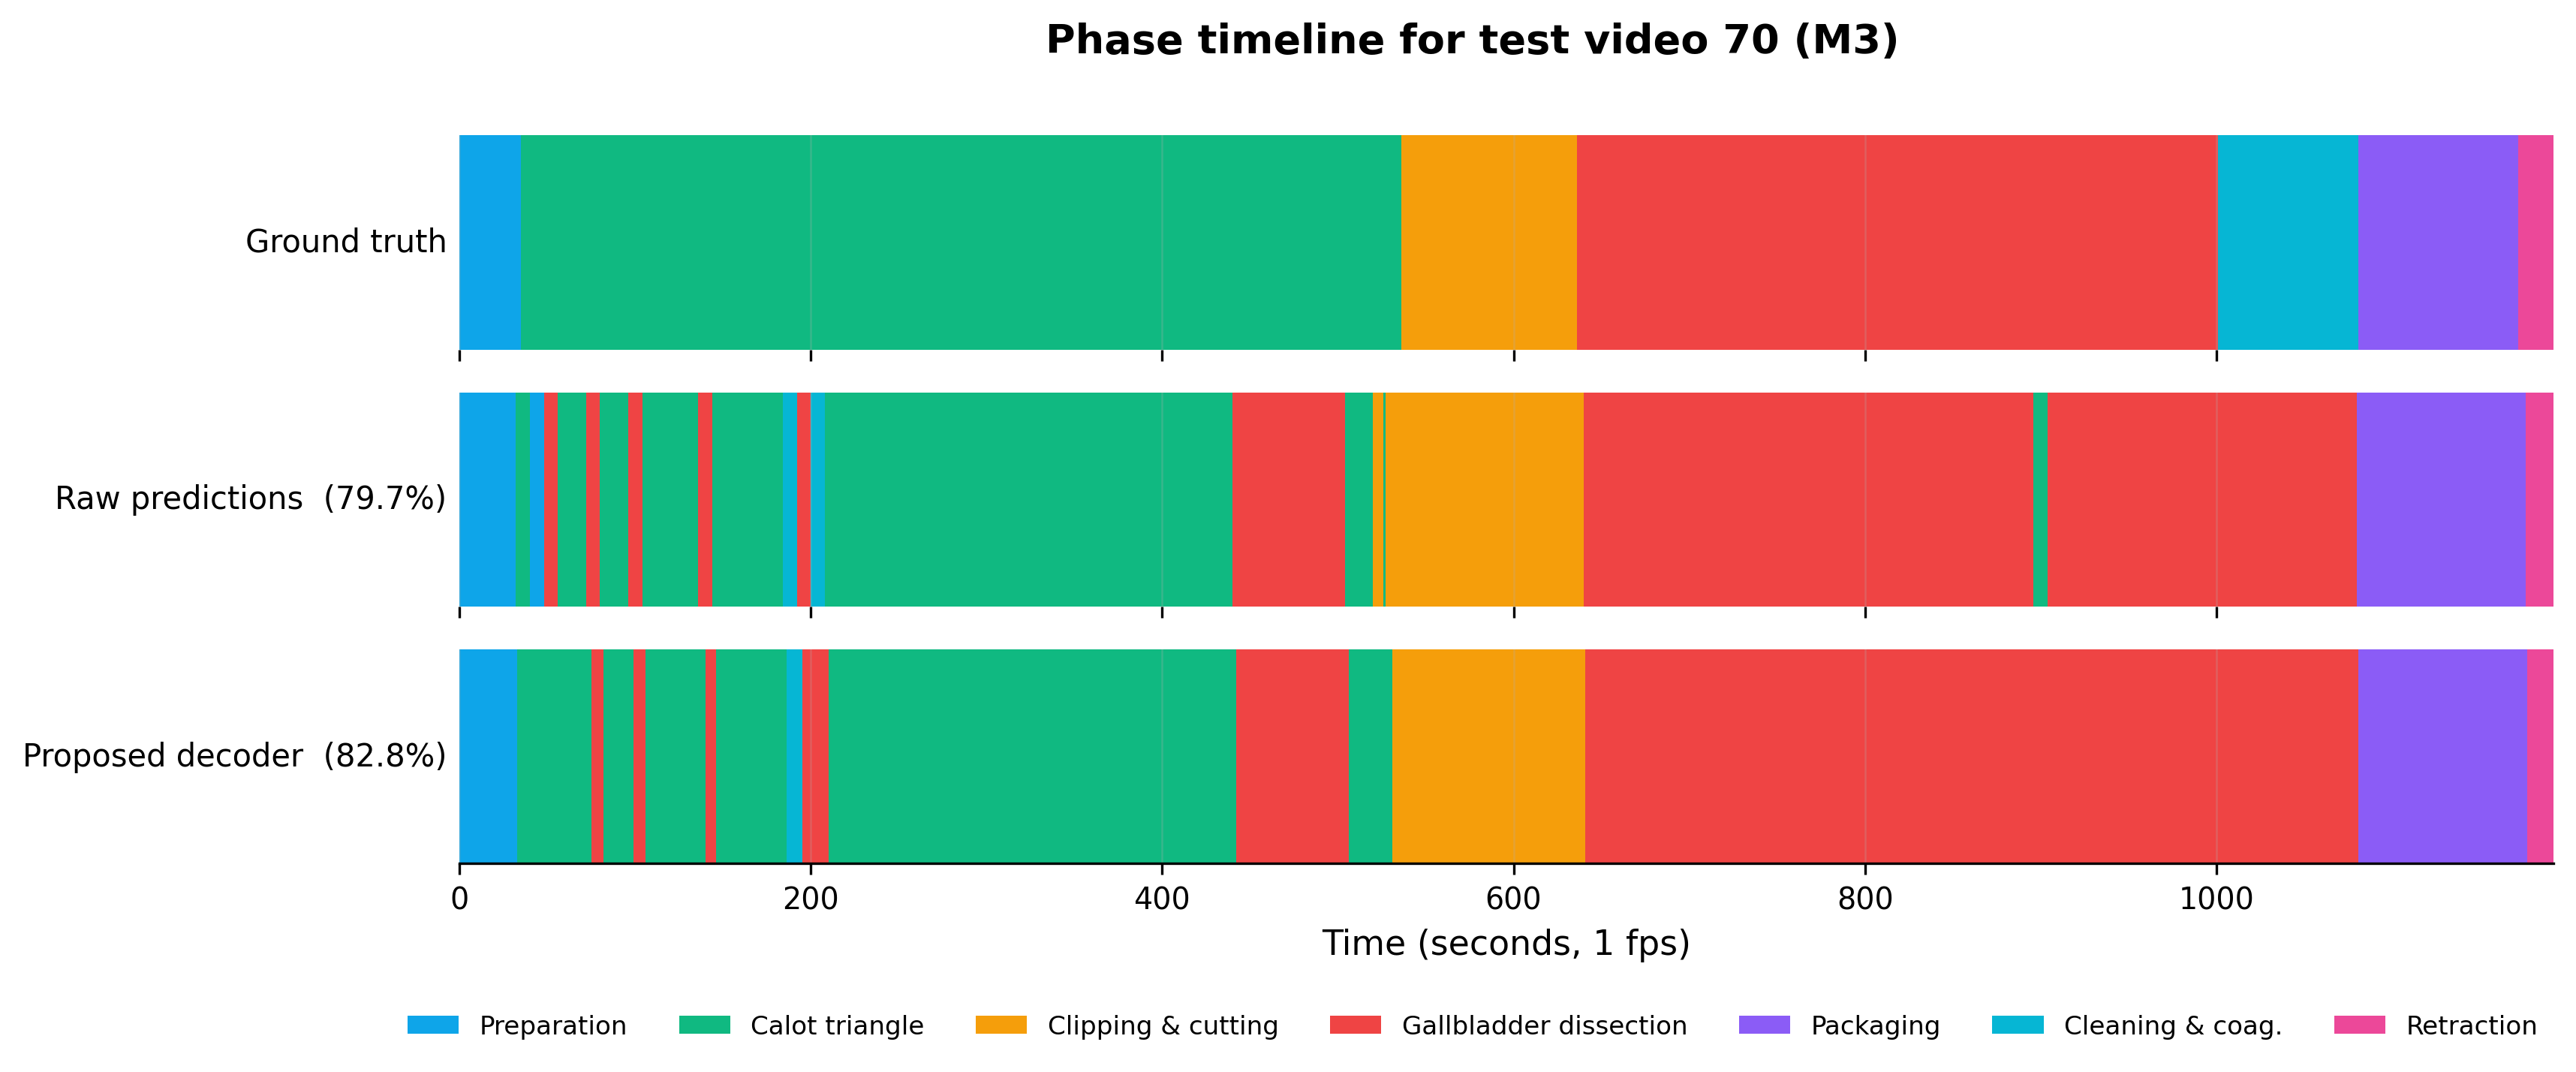
\includegraphics[width=\textwidth]{figures/timeline.png}
\caption{Phase timeline for one test video (M3). The raw predictions (middle) flip often; the proposed decoder (bottom) is much smoother and stays close to the ground truth (top).}
\label{fig:timeline}
\end{figure}

\section{Errors Near Phase Changes versus Inside Phases}
\label{sec:boundary}

On Cholec80, label disagreement is concentrated at the phase changes, where even human annotators differ on the exact moment of transition. To see where each decoder helps, the test frames are split into those \textbf{near a phase change} (within $\pm5$~s of a true transition) and those \textbf{inside a phase} (everywhere else). Table~\ref{tab:boundary} reports the split for M3, and Figure~\ref{fig:boundary} shows it.

\begin{table}[H]
\centering
\caption{Accuracy near phase changes versus inside phases, for M3. The offline decoder $\dagger$ uses future frames. Best \emph{real-time} values in \textbf{bold}.}
\label{tab:boundary}
\begin{tabular}{lcc}
\toprule
\textbf{Decoder} & \textbf{Near change} & \textbf{Inside phase} \\
\midrule
Raw predictions          & 60.7\% & 86.1\% \\
Median-15 filter         & 61.1\% & 86.3\% \\
\textbf{Proposed decoder} & \textbf{63.2\%} & 86.8\% \\
\midrule
Offline (full video) $\dagger$ & 62.8\% & 91.0\% \\
\bottomrule
\end{tabular}
\end{table}

\begin{figure}[H]
\centering
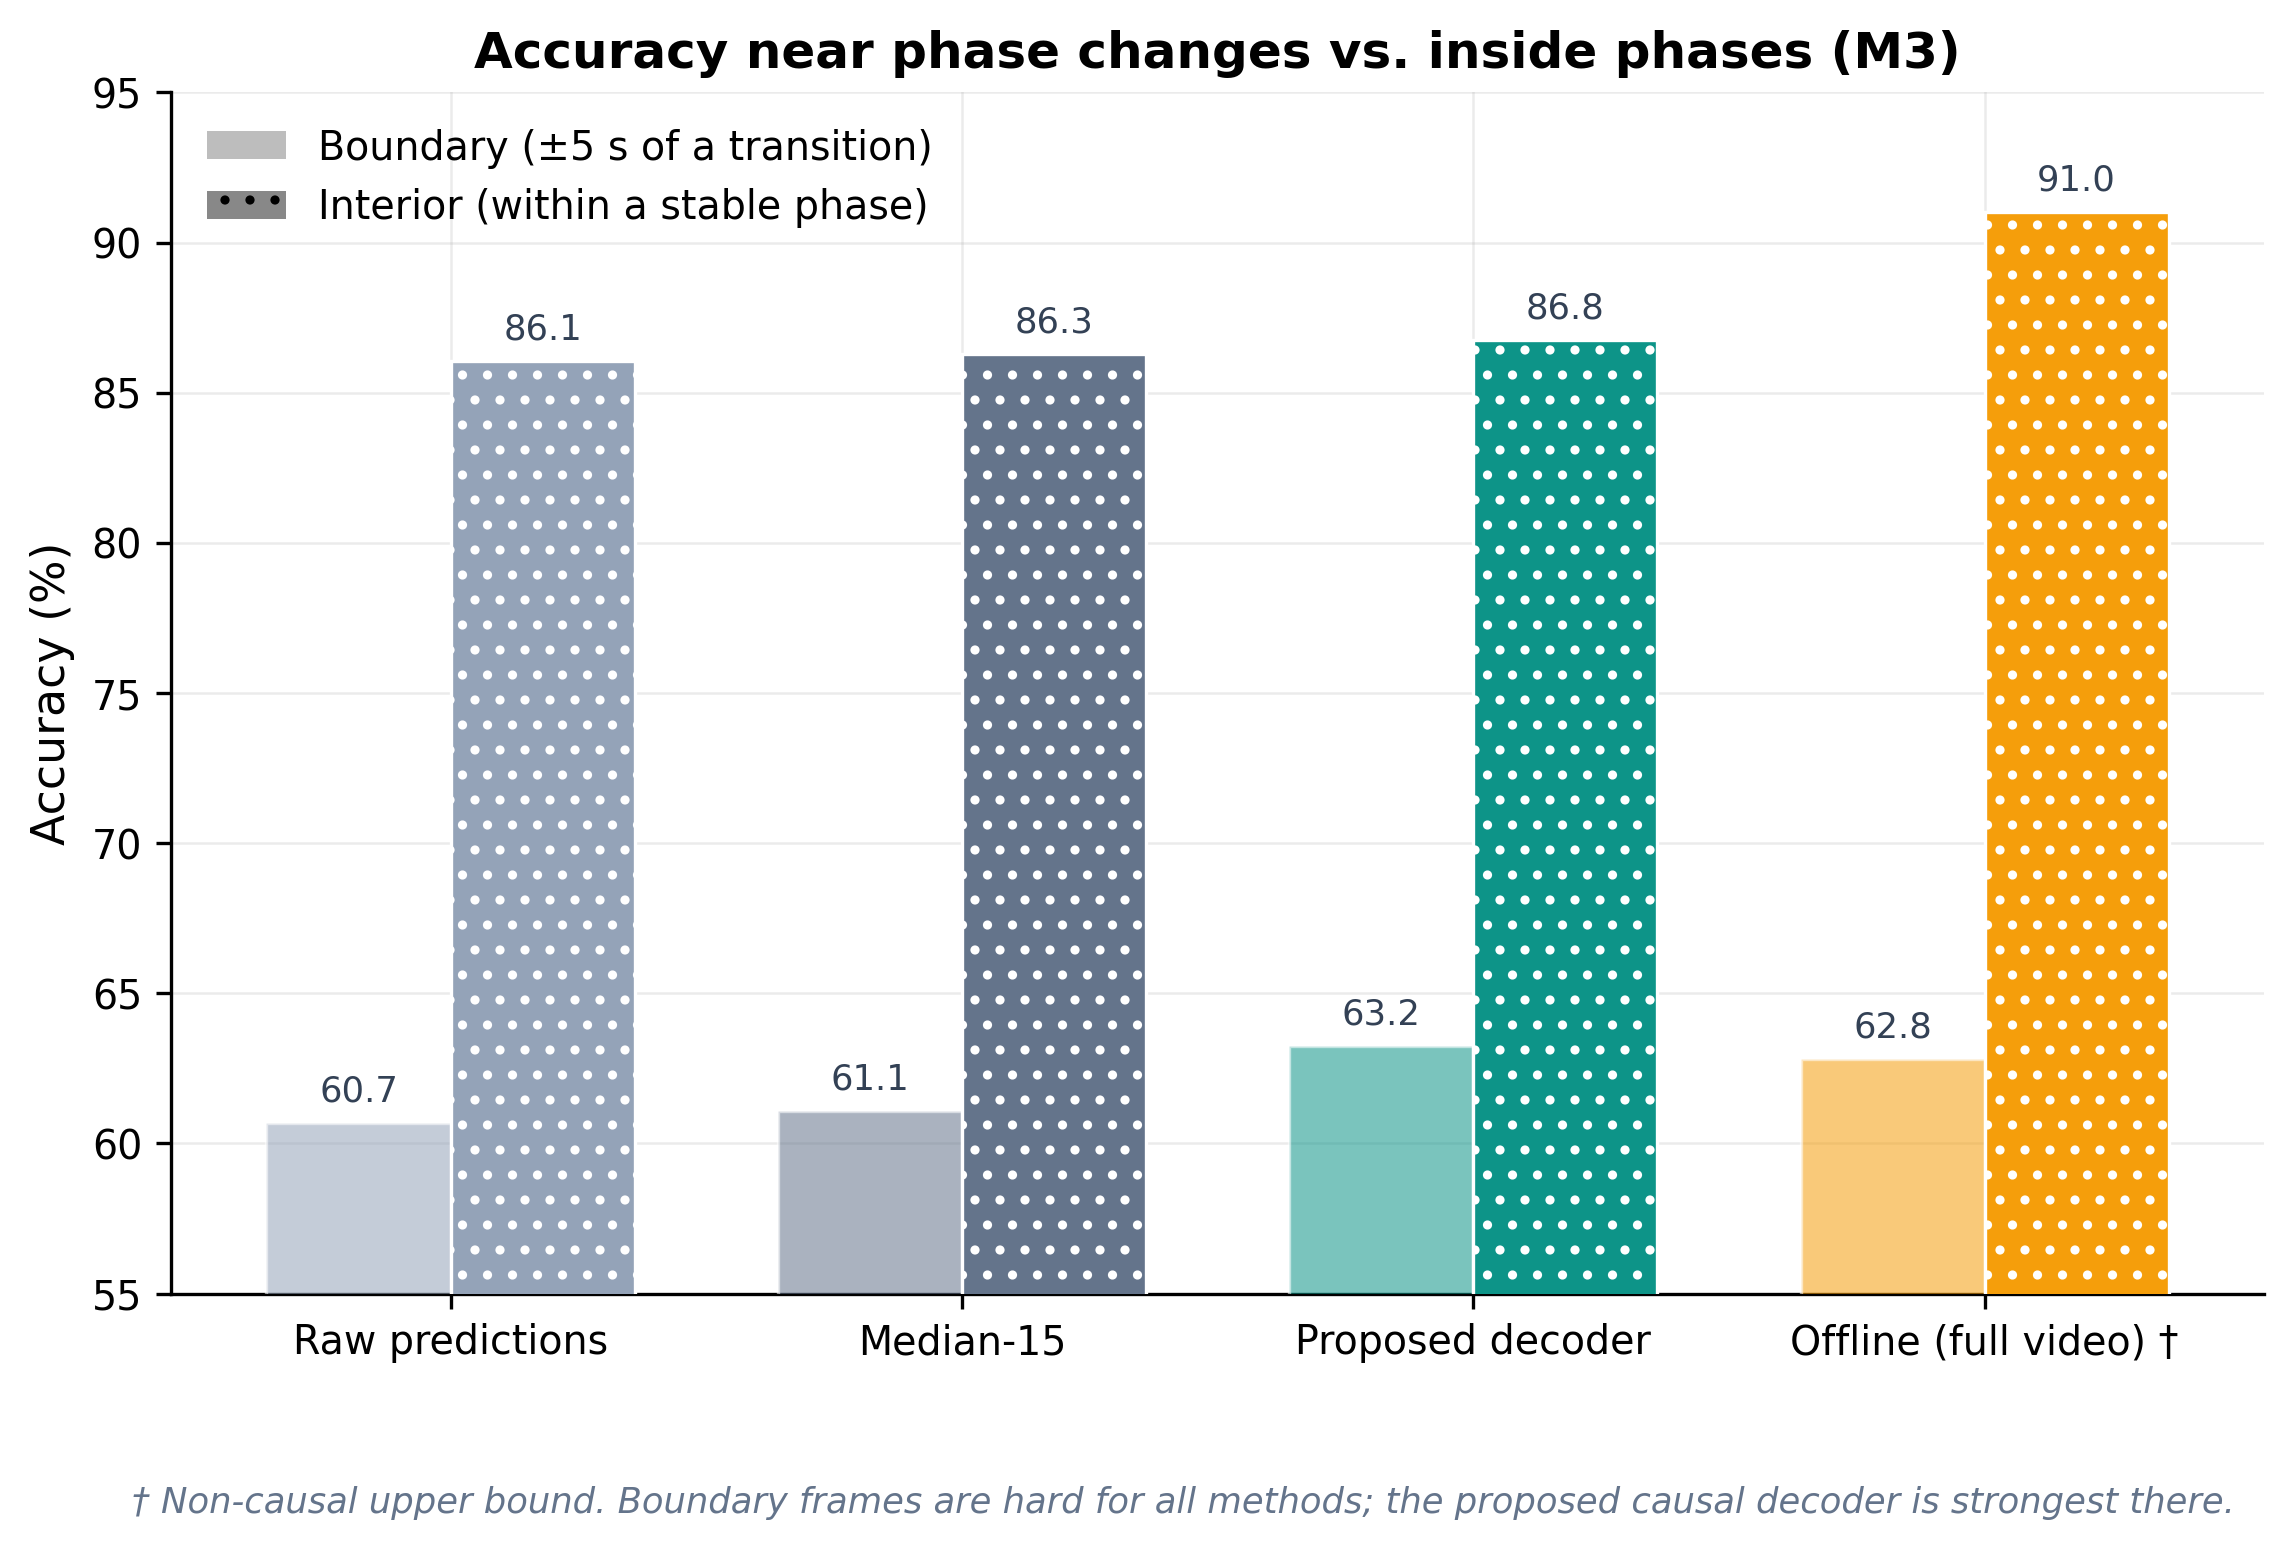
\includegraphics[width=\figwidth]{figures/boundary.png}
\caption{Accuracy near phase changes versus inside phases, for M3. Frames near a change (solid bars) are hard for every method; the proposed decoder is best there, even slightly above the offline upper bound. Inside phases (hatched bars) is where the offline decoder's advantage comes from.}
\label{fig:boundary}
\end{figure}

Two points stand out. First, the proposed decoder is the \textbf{best near phase changes} (63.2\%), even above the offline upper bound (62.8\%): the offline decoder's hard rule that phases cannot go backwards sometimes delays a transition, while the soft learned table follows the labelled timing more flexibly. Second, the whole 4.2-point gap between the offline decoder and the best real-time decoder is \emph{inside} the phases ($86.8 \to 91.0$), not at the changes. The offline decoder's advantage is fixing brief mistakes inside long stable phases by looking at future frames---something a real-time decoder cannot do. To our knowledge this split has not been measured before on Cholec80, and it points to a clear next step: letting the decoder look a few seconds ahead would close most of the gap while still being usable in near-real time.

% ======================= CHAPTER 5: CONCLUSION ==========================
\chapter{Conclusion and Future Work}

\section{Summary of Contributions}

This thesis studied surgical phase recognition on Cholec80 on a single laptop GPU, around two connected parts.

The first is a \textbf{fair comparison of three architectures}. ResNet-50~+~BiLSTM, EfficientNet-B3~+~TCN, and Swin-Tiny~+~Transformer were trained with one identical pipeline (a three-stage schedule, class re-weighting, the extra tool task, label smoothing, and mixed-precision training) on a single 4~GB GPU. Keeping the recipe fixed isolates the effect of the architecture: the Swin-Transformer reached a smoothed macro-F1 of 0.815, 3.4 points above the ResNet-LSTM and 6.7 above the EfficientNet-TCN. Four ablations then showed the tool task is worth about $+1.6\%$ macro-F1 and class re-weighting about $+2.0\%$, and combining the three models added another 1.0 point.

The second part is about the \textbf{decoding and calibration steps} that most Cholec80 work skips. A real-time decoder, combining temperature-calibrated predictions with a learned transition table, was added. Without retraining the models, it raised test accuracy by $+0.6$ to $+1.7$ points across the three models---a small but, by the paired test, clear and consistent gain---at a cost of 0.013~ms per frame. Splitting the errors showed the decoder is strongest exactly where the models are weakest (at phase changes), and that the remaining gap to the offline upper bound is entirely inside the phases.

\section{Key Findings}

Three findings go beyond the specific dataset and models studied.

\textbf{The training recipe matters as much as the architecture.} Class weighting and the tool task together are worth almost four points of macro-F1---about the same as the gap between the best and worst architecture. On an imbalanced surgical dataset, how the model is trained is as important as which backbone is used. This is easy to miss when a comparison changes the architecture and the recipe at the same time, which is exactly what the fixed pipeline here was meant to avoid.

\textbf{Calibration is what makes the transition table useful.} Temperature scaling is usually justified by trust alone, but it has a second role here: the decoder adds the calibrated scores and the transition weights together, so if the scores are too sharp the table is ignored. Calibrating the scores is what lets the learned phase order help, which is why the calibrated decoder consistently beats the uncalibrated one.

\textbf{The benefit of looking ahead is inside the phases.} The offline decoder's advantage over the best real-time decoder is almost entirely about fixing brief mistakes inside long, stable phases using future frames---not about placing the phase changes more precisely. So a real-time system gives up the ability to fix those interior glitches, not boundary accuracy. Letting the decoder look a few seconds ahead is therefore the natural next step.

\section{Limitations}

Several constraints bound the conclusions of this study:

\begin{itemize}
    \item \textbf{Limited hardware.} The 4~GB GPU forced a small batch size and sequence length. Results on larger hardware would likely be one to three points higher, and the EfficientNet-TCN in particular had its Stage-3 fine-tuning cut short, so its numbers are a lower bound rather than a fair estimate.
    \item \textbf{One dataset.} All results are from Cholec80. Procedures with a less strict phase order may need a looser transition table, and transfer to other surgeries is untested.
    \item \textbf{Label noise at phase changes.} The exact moment of each phase change in Cholec80 is imprecise, which caps the achievable accuracy near phase changes; this cap is not measured here.
    \item \textbf{Sub-sampling in the live demo.} The interactive demo skips frames for speed, so short closing phases can be missed at low sampling rates. The reported benchmark numbers use the full 1~fps protocol and are not affected.
\end{itemize}

\section{Future Work}

The most direct extensions address these limitations:

\begin{itemize}
    \item \textbf{A short look-ahead.} A decoder allowed to look a few seconds ahead would recover most of the gap inside phases while keeping the delay small, addressing the bottleneck found in Section~\ref{sec:boundary}.
    \item \textbf{Re-training on larger hardware.} Running the same three architectures with a larger batch and longer sequences would show how much of the gap to the best published results is due to hardware rather than the architecture.
    \item \textbf{Uncertainty estimates.} Adding Monte-Carlo dropout or ensemble-based uncertainty, on top of the calibration already done, would give each prediction a confidence value that a clinician could use.
    \item \textbf{Other procedures.} Re-training on other surgeries with workflow labels would test whether the pipeline and the learned-table decoder work beyond cholecystectomy.
\end{itemize}

In summary, this thesis shows that good surgical phase recognition is possible on an ordinary laptop GPU when training, decoding, and post-processing are designed together---and that the decoding and calibration steps, often treated as an afterthought, give a real, measurable, real-time improvement.


% ======================= REFERENCES ==========================
\printbibliography[title={References}]

\end{document}
